\documentclass[12pt]{article}
%DIF LATEXDIFF DIFFERENCE FILE
%DIF DEL old.tex   Sat Oct 10 00:54:32 2026
%DIF ADD new.tex   Sat Oct 10 01:57:14 2026

\usepackage{graphicx}
\usepackage{caption}
\usepackage{amsmath, amssymb, amsthm}
\usepackage{booktabs}
\usepackage{enumitem}
\usepackage{geometry}
\geometry{margin=1in}
\usepackage{xcolor}
\usepackage{float}
%DIF 12-14d12
%DIF < % \usepackage[numbers,sort&compress]{natbib} % number style
%DIF < \usepackage[colorlinks=true, allcolors=blue]{hyperref} %For hyperlinks, usually must be the last package called
%DIF < \usepackage[capitalise]{cleveref} % must be loaded after hyperef
%DIF -------
\usepackage{tabularx}
%DIF 16d13
%DIF < \usepackage{float}
%DIF -------
\usepackage[normalem]{ulem} % normalem keeps \emph working normally
%DIF 18-22d14
%DIF < 
%DIF < 
%DIF < 
%DIF < 
%DIF < % Packages for algorithms and pseudocode
%DIF -------
\usepackage{algorithm}
\usepackage{algpseudocode}
%DIF 25a16-17
\usepackage[colorlinks=true, allcolors=blue]{hyperref} % load near the end
 %DIF > 
\usepackage[capitalise]{cleveref} % must be loaded after hyperref
 %DIF > 
%DIF -------

\title{NPSC3000 End of Year Report: Can Reinforcement Learning Outperform Traditional Methods for Cloud Resource Allocation}
\author{
\textbf{Student:} Ty Riekert \\
\textbf{Supervisor:} Elham Mardaneh \\
\textbf{Co-supervisor:} Tony Mathew
}
\date{\DIFdelbegin \DIFdel{Sept }\DIFdelend \DIFaddbegin \DIFadd{October }\DIFaddend 2026}
%DIF 33-34d26
%DIF < 
%DIF < 
%DIF -------

%DIF PREAMBLE EXTENSION ADDED BY LATEXDIFF
%DIF PREAMBLE: new or changed text in red, deleted text hidden
\RequirePackage{xcolor} %DIF PREAMBLE
\providecommand{\DIFaddtex}[1]{{\color{red}#1}} %DIF PREAMBLE
\providecommand{\DIFdeltex}[1]{} %DIF PREAMBLE
\providecommand{\DIFaddbegin}{} %DIF PREAMBLE
\providecommand{\DIFaddend}{} %DIF PREAMBLE
\providecommand{\DIFdelbegin}{} %DIF PREAMBLE
\providecommand{\DIFdelend}{} %DIF PREAMBLE
\providecommand{\DIFmodbegin}{} %DIF PREAMBLE
\providecommand{\DIFmodend}{} %DIF PREAMBLE
\providecommand{\DIFaddFL}[1]{{\color{red}#1}} %DIF PREAMBLE
\providecommand{\DIFdelFL}[1]{} %DIF PREAMBLE
\providecommand{\DIFaddbeginFL}{} %DIF PREAMBLE
\providecommand{\DIFaddendFL}{} %DIF PREAMBLE
\providecommand{\DIFdelbeginFL}{} %DIF PREAMBLE
\providecommand{\DIFdelendFL}{} %DIF PREAMBLE
%DIF END PREAMBLE %DIF PREAMBLE
%DIF HYPERREF PREAMBLE %DIF PREAMBLE
\providecommand{\DIFadd}[1]{\texorpdfstring{\DIFaddtex{#1}}{#1}} %DIF PREAMBLE
\providecommand{\DIFdel}[1]{\texorpdfstring{\DIFdeltex{#1}}{}} %DIF PREAMBLE
\providecommand{\DIFscaledelfig}{0.5}
%DIF HIGHLIGHTGRAPHICS PREAMBLE %DIF PREAMBLE
\RequirePackage{settobox} %DIF PREAMBLE
\RequirePackage{letltxmacro} %DIF PREAMBLE
\newsavebox{\DIFdelgraphicsbox} %DIF PREAMBLE
\newlength{\DIFdelgraphicswidth} %DIF PREAMBLE
\newlength{\DIFdelgraphicsheight} %DIF PREAMBLE
% store original definition of \includegraphics %DIF PREAMBLE
\LetLtxMacro{\DIFOincludegraphics}{\includegraphics} %DIF PREAMBLE
\providecommand{\DIFaddincludegraphics}[2][]{{\color{blue}\fbox{\DIFOincludegraphics[#1]{#2}}}} %DIF PREAMBLE
\providecommand{\DIFdelincludegraphics}[2][]{% %DIF PREAMBLE
\sbox{\DIFdelgraphicsbox}{\DIFOincludegraphics[#1]{#2}}% %DIF PREAMBLE
\settoboxwidth{\DIFdelgraphicswidth}{\DIFdelgraphicsbox} %DIF PREAMBLE
\settoboxtotalheight{\DIFdelgraphicsheight}{\DIFdelgraphicsbox} %DIF PREAMBLE
\scalebox{\DIFscaledelfig}{% %DIF PREAMBLE
\parbox[b]{\DIFdelgraphicswidth}{\usebox{\DIFdelgraphicsbox}\\[-\baselineskip] \rule{\DIFdelgraphicswidth}{0em}}\llap{\resizebox{\DIFdelgraphicswidth}{\DIFdelgraphicsheight}{% %DIF PREAMBLE
\setlength{\unitlength}{\DIFdelgraphicswidth}% %DIF PREAMBLE
\begin{picture}(1,1)% %DIF PREAMBLE
\thicklines\linethickness{2pt} %DIF PREAMBLE
{\color[rgb]{1,0,0}\put(0,0){\framebox(1,1){}}}% %DIF PREAMBLE
{\color[rgb]{1,0,0}\put(0,0){\line( 1,1){1}}}% %DIF PREAMBLE
{\color[rgb]{1,0,0}\put(0,1){\line(1,-1){1}}}% %DIF PREAMBLE
\end{picture}% %DIF PREAMBLE
}\hspace*{3pt}}} %DIF PREAMBLE
} %DIF PREAMBLE
\LetLtxMacro{\DIFOaddbegin}{\DIFaddbegin} %DIF PREAMBLE
\LetLtxMacro{\DIFOaddend}{\DIFaddend} %DIF PREAMBLE
\LetLtxMacro{\DIFOdelbegin}{\DIFdelbegin} %DIF PREAMBLE
\LetLtxMacro{\DIFOdelend}{\DIFdelend} %DIF PREAMBLE
\DeclareRobustCommand{\DIFaddbegin}{\DIFOaddbegin \let\includegraphics\DIFaddincludegraphics} %DIF PREAMBLE
\DeclareRobustCommand{\DIFaddend}{\DIFOaddend \let\includegraphics\DIFOincludegraphics} %DIF PREAMBLE
\DeclareRobustCommand{\DIFdelbegin}{\DIFOdelbegin \let\includegraphics\DIFdelincludegraphics} %DIF PREAMBLE
\DeclareRobustCommand{\DIFdelend}{\DIFOaddend \let\includegraphics\DIFOincludegraphics} %DIF PREAMBLE
\LetLtxMacro{\DIFOaddbeginFL}{\DIFaddbeginFL} %DIF PREAMBLE
\LetLtxMacro{\DIFOaddendFL}{\DIFaddendFL} %DIF PREAMBLE
\LetLtxMacro{\DIFOdelbeginFL}{\DIFdelbeginFL} %DIF PREAMBLE
\LetLtxMacro{\DIFOdelendFL}{\DIFdelendFL} %DIF PREAMBLE
\DeclareRobustCommand{\DIFaddbeginFL}{\DIFOaddbeginFL \let\includegraphics\DIFaddincludegraphics} %DIF PREAMBLE
\DeclareRobustCommand{\DIFaddendFL}{\DIFOaddendFL \let\includegraphics\DIFOincludegraphics} %DIF PREAMBLE
\DeclareRobustCommand{\DIFdelbeginFL}{\DIFOdelbeginFL \let\includegraphics\DIFdelincludegraphics} %DIF PREAMBLE
\DeclareRobustCommand{\DIFdelendFL}{\DIFOaddendFL \let\includegraphics\DIFOincludegraphics} %DIF PREAMBLE
%DIF AMSMATHULEM PREAMBLE %DIF PREAMBLE
\makeatletter %DIF PREAMBLE
\let\sout@orig\sout %DIF PREAMBLE
\renewcommand{\sout}[1]{\ifmmode\text{\sout@orig{\ensuremath{#1}}}\else\sout@orig{#1}\fi} %DIF PREAMBLE
\makeatother %DIF PREAMBLE
%DIF LISTINGS PREAMBLE %DIF PREAMBLE
\RequirePackage{listings} %DIF PREAMBLE
\lstdefinelanguage{DIFcode}{ %DIF PREAMBLE
%DIF DIFCODE_BOLD %DIF PREAMBLE
  % unfortunately \bfseries cannot be combined with ttfamily without extra packages %DIF PREAMBLE
  % also morecomment=[il] is broken as of v1.5b of listings at least %DIF PREAMBLE
  % workaround: plot in white with tiny font %DIF PREAMBLE
  % morecomment=[il]{\%DIF\ <\ }, %DIF PREAMBLE
  moredelim=[il][\color{white}\tiny]{\%DIF\ <\ }, %DIF PREAMBLE
  moredelim=[il][\sffamily\bfseries]{\%DIF\ >\ } %DIF PREAMBLE
} %DIF PREAMBLE
\lstdefinestyle{DIFverbatimstyle}{ %DIF PREAMBLE
	language=DIFcode, %DIF PREAMBLE
	basicstyle=\ttfamily, %DIF PREAMBLE
	columns=fullflexible, %DIF PREAMBLE
	keepspaces=true %DIF PREAMBLE
} %DIF PREAMBLE
\lstnewenvironment{DIFverbatim}[1][]{\lstset{style=DIFverbatimstyle,#1}}{} %DIF PREAMBLE
\lstnewenvironment{DIFverbatim*}[1][]{\lstset{style=DIFverbatimstyle,showspaces=true,#1}}{} %DIF PREAMBLE
\lstset{extendedchars=\true,inputencoding=utf8}

%DIF END PREAMBLE EXTENSION ADDED BY LATEXDIFF

\begin{document}
\maketitle

\DIFaddbegin 

%DIF >  =====================================================================
\DIFaddend \begin{abstract}
\DIFdelbegin \DIFdel{The problem of resource }\DIFdelend \DIFaddbegin \DIFadd{Resource }\DIFaddend allocation (RA) is a critical \DIFdelbegin \DIFdel{issue amongst }\DIFdelend \DIFaddbegin \DIFadd{problem for }\DIFaddend cloud providers \cite{saidi2023, sdn2021, vinothina2012, parikh2013, mohamaddiah2014}\DIFdelbegin \DIFdel{. There exists a shared set of physical resources such as servers , network, storage, and user applications that they need to manage in real-time. These resources are dynamically managed and allocated in the form of jobs to virtual machines (VMs), and it's a vital challenge to ensure operations, traffic performance, and energy conservation of these VMS are properly managed. One approach in which this can be modelled is as a Resource-Constrained Project Scheduling (RCS) optimisation problem. With user applications and jobs arriving in real-time, this problem is considered to be online in that the overall decision horizon for algorithms to assign jobs to machines is non-deterministic. Since cloud RA is also inherently a multi-objective and dynamic problem, traditional methods have been shown to struggle \mbox{%DIFAUXCMD
\cite{lbts2024, 10854610, DAHMANI2025100616, DBLP:journals/corr/abs-2107-04333}}\hskip0pt%DIFAUXCMD
, however, recent studies highlight the strong potential of }\DIFdelend \DIFaddbegin \DIFadd{: a shared pool of physical servers must serve a continuous stream of user jobs while meeting deadlines and limiting energy use. Classical scheduling methods are known to struggle with the dynamic, multi-objective nature of this problem \mbox{%DIFAUXCMD
\cite{lbts2024, 10854610, DAHMANI2025100616}}\hskip0pt%DIFAUXCMD
, while }\DIFaddend reinforcement learning (RL) \DIFdelbegin \DIFdel{in handling dynamic and large-scale environments reflected in such a problem }\DIFdelend \DIFaddbegin \DIFadd{has shown promise in similar settings }\DIFaddend \cite{saidi2023, autoscaling2023, lbts2024, dynamic2026}. \DIFdelbegin \DIFdel{Building on the insights of such papers, this report aims to implement a reinforcement learning agent that can outperform traditional methods on the comparison of tardiness, late and assigned jobs , and total objective reward. Versions and iterations of two RL approaches were implemented: }\DIFdelend \DIFaddbegin \DIFadd{This project asks }\emph{\DIFadd{under which objectives and conditions RL outperforms classical scheduling methods}}\DIFadd{. We model cloud RA as a multi-resource scheduling problem in two settings, offline (all jobs known in advance) and online (jobs arrive randomly), and formulate it as a Markov decision process. Six action-space designs were trained with }\DIFaddend proximal policy optimisation (PPO) and advantage \DIFdelbegin \DIFdel{actor critic }\DIFdelend \DIFaddbegin \DIFadd{actor-critic }\DIFaddend (A2C) \DIFdelbegin \DIFdel{agents. Preliminary results on the offline scheduling case show PPO fails to learn useful assignments under every configuration tested (reward tuning , hyperparameter search, Lagrangian, and pointer-network architecture alike), converging to tardiness which is statistically indistinguishable from heuristics that ignore deadlines entirely. In contrast, A2C with potential-based reward shaping \mbox{%DIFAUXCMD
\cite{ng1999shaping} }\hskip0pt%DIFAUXCMD
achieves results competitive with a few heuristic baselines on the fixed data instance setting, althought on a randomized set of instances, all RL models fail to obtain meaningful results. \textcolor{red}{In the online setting with stochastic job arrivals, the RL agent with action-space overhaulingly outperforms the majority of the heuristics in some architectures, with less than average in other iterations}. Fully closing the gap between RL and heuristic or rule-based policies is still under work.
}%DIFDELCMD < 

%DIFDELCMD < %%%
\DIFdelend \DIFaddbegin \DIFadd{under one uniform tuning and training protocol, and compared on 50 held-out instances against 49 dispatching heuristics and the CP-SAT exact solver. On the main objective, weighted squared tardiness, the best RL agent comes within 5\% of the best heuristic offline but does not beat it, and only ties the best heuristic when all jobs are equally important. Once linear tardiness or the number of late jobs is added to the objective, RL beats the best heuristic by 2--10\% offline. Online, RL needs far more training: with more steps the best design closed most of its gap to the best heuristic but did not overtake it. RL never beat the heuristics when energy was part of the objective. Overall, RL is most competitive when the objective combines several goals that no single hand-designed rule targets, and when jobs differ in importance.
}\DIFaddend \end{abstract}

\newpage
%DIF >  =====================================================================
\section{Project \DIFaddbegin \DIFadd{Aims and }\DIFaddend Deliverables}
The aim of this project is to formulate cloud resource allocation as a mathematical optimisation and reinforcement learning problem\DIFdelbegin \DIFdel{. Implementing and rigorously evaluating }\DIFdelend \DIFaddbegin \DIFadd{, and to rigorously evaluate }\DIFaddend RL models against established methods. The specific deliverables are:
\begin{itemize}
    \item Conduct comprehensive research on current findings and machine learning in cloud resource allocation
    \item Formulate a mathematical model of the cloud RA problem, expressed as a resource-constrained scheduling optimisation problem
    \item Create a corresponding Markov Decision Process (MDP) formulation \DIFdelbegin \DIFdel{of }\DIFdelend \DIFaddbegin \DIFadd{for }\DIFaddend the reinforcement learning agent
    \item Implement the code of the scheduling environment
    \item Implement the code for the reinforcement learning agent(s)
    \item Evaluate the trained agents against classical scheduling heuristics to determine under what conditions reinforcement learning outperforms traditional methods.
\end{itemize}
The last item is not \DIFdelbegin \DIFdel{done with }\DIFdelend a single `train and compare' run, but \DIFdelbegin \DIFdel{is }\DIFdelend an iterative process repeated throughout the \DIFdelbegin \DIFdel{entire last }\DIFdelend \DIFaddbegin \DIFadd{second }\DIFaddend half of the project\DIFdelbegin \DIFdel{. A }\DIFdelend \DIFaddbegin \DIFadd{: a }\DIFaddend constant loop of training, evaluating against baselines, \DIFdelbegin \DIFdel{examining and researching }\DIFdelend \DIFaddbegin \DIFadd{investigating }\DIFaddend behaviour and faults, \DIFaddbegin \DIFadd{checking them against the literature, }\DIFaddend and revising.

%DIF >  =====================================================================
\section{Background}
\subsection{Cloud Computing}
Cloud computing refers to the use of computing services and resources delivered over the internet, and resource allocation (RA) is one of the most critical challenges facing cloud providers today \cite{saidi2023, huawei2022}. As cloud infrastructure underpins the majority of modern computing services, effectively allocating physical resources, like compute or network bandwidth\DIFaddbegin \DIFadd{, }\DIFaddend to a continuously arriving stream of workloads \DIFdelbegin \DIFdel{, }\DIFdelend has become of vital importance to providers \cite{sdn2021}. Poor allocation \DIFdelbegin \DIFdel{can lead to poor metrics in }\DIFdelend \DIFaddbegin \DIFadd{leads to poor }\DIFaddend response time, \DIFdelbegin \DIFdel{environmental sustainability, energy or power efficiency, }\DIFdelend throughput, makespan, utilisation\DIFdelbegin \DIFdel{and more }\DIFdelend \DIFaddbegin \DIFadd{, energy efficiency and environmental sustainability }\DIFaddend \cite{cloudkpi2010, dvbpp2026, mohamaddiah2014, anuradha2014}.

\subsubsection{Cloud RA}
Cloud RA can be decomposed into several coupled problems. Virtual machine (VM) placement \DIFdelbegin \DIFdel{takes the cloud provider's physical servers as virtual machines subject to resource constraints like CPUand memory . User requests are then assigned to those virtual machines. This }\DIFdelend \DIFaddbegin \DIFadd{decides which physical server hosts each virtual machine, subject to the server's CPU, memory and other capacities, and }\DIFaddend is widely regarded as the core RA subproblem \cite{saidi2023}. Task scheduling \DIFdelbegin \DIFdel{divides the workload evenly across all available resources while minimising execution and response time}\DIFdelend \DIFaddbegin \DIFadd{decides when and on which resource each user task runs; depending on the setting it may prioritise execution time, response time, deadlines or an even spread of work }\DIFaddend \cite{lbts2024}. Autoscaling dynamically adjusts resource capacity to match fluctuating demand \DIFdelbegin \DIFdel{in real time }\DIFdelend \cite{autoscaling2023}, and load balancing distributes incoming tasks evenly to avoid hotspots \cite{lb2024}. \DIFdelbegin %DIFDELCMD < \newline
%DIFDELCMD < %%%
\DIFdelend \DIFaddbegin \DIFadd{This project studies the task-scheduling view: deciding when and where each job runs.

}

\DIFaddend Solutions to these problems generally fall into three categories\DIFaddbegin \DIFadd{:
}\DIFaddend \begin{itemize}
    \item \textbf{Exact \DIFdelbegin \DIFdel{Methods}%DIFDELCMD < \MBLOCKRIGHTBRACE%%%
\DIFdel{. Algorithmsthat always solve a problem optimally
    }\DIFdelend \DIFaddbegin \DIFadd{methods.}} \DIFadd{Algorithms, such as integer and constraint programming, that are guaranteed to find an optimal solution given enough time.
    }\DIFaddend \item \DIFdelbegin \textbf{\DIFdel{Approximation Methods}}%DIFAUXCMD
\DIFdel{. These methods are used when exact algorithms }\DIFdelend \DIFaddbegin \textbf{\DIFadd{Approximation methods.}} \DIFadd{Used when exact methods }\DIFaddend become computationally infeasible. \DIFdelbegin \DIFdel{Two main classes are heuristics which algorithms design to }\DIFdelend \DIFaddbegin \emph{\DIFadd{Heuristics}} \DIFadd{are problem-specific rules, designed by people from domain knowledge, that }\DIFaddend quickly construct or improve a single solution \DIFdelbegin \DIFdel{, and metaheuristics that are more higher-level and }\DIFdelend \DIFaddbegin \DIFadd{(for example, ``always run the job with the earliest deadline''). }\emph{\DIFadd{Metaheuristics}} \DIFadd{are general-purpose search strategies, such as particle swarm optimisation, that }\DIFaddend guide heuristic methods \DIFdelbegin \DIFdel{in a strategic manner \mbox{%DIFAUXCMD
\cite{alkhalifa2025comparative}}\hskip0pt%DIFAUXCMD
}\DIFdelend \DIFaddbegin \DIFadd{through the space of solutions \mbox{%DIFAUXCMD
\cite{alkhalifa2025comparative}}\hskip0pt%DIFAUXCMD
.
    }\DIFaddend \item \DIFdelbegin \textbf{\DIFdel{Machine learning}}%DIFAUXCMD
\DIFdel{.
    Algorithms that are based on enforcing a set of rules to get the machine to learn on data
}\DIFdelend \DIFaddbegin \textbf{\DIFadd{Machine learning (ML).}} \DIFadd{Methods that learn a decision rule from data or experience instead of having it written by hand. For scheduling, a model is trained on many example problems, and the trained model then makes allocation decisions on new problems.
}\DIFaddend \end{itemize}

Exact methods guarantee optimality\DIFdelbegin \DIFdel{on }\DIFdelend \DIFaddbegin \DIFadd{, but scheduling problems of this kind are NP-hard \mbox{%DIFAUXCMD
\cite{lenstra1977complexity}}\hskip0pt%DIFAUXCMD
, so their run time grows rapidly with problem size; in practice they are limited to }\DIFaddend small instances, \DIFdelbegin \DIFdel{scale terribly, and are then only useful for lower bound estimates}\DIFdelend \DIFaddbegin \DIFadd{or are stopped early and used for the best solution and bounds they have found}\DIFaddend . Heuristics and metaheuristics scale well \DIFdelbegin \DIFdel{, but can yield approximate solution that may not be sufficiently accurate}\DIFdelend \DIFaddbegin \DIFadd{but give approximate solutions with no guarantee of quality}\DIFaddend . Systematic reviews \DIFdelbegin \DIFdel{within this field identify four major problems }\DIFdelend \DIFaddbegin \DIFadd{identify four recurring limitations }\DIFaddend of these approximation methods \DIFdelbegin \DIFdel{: scalability, adaptability, generalisation multi-objective complexity, high computational cost with scale, and }\DIFdelend \DIFaddbegin \DIFadd{in cloud RA: scalability to large systems, adaptability to changing workloads, handling several conflicting objectives at once, and the need for }\DIFaddend real-time \DIFdelbegin \DIFdel{decision making }\DIFdelend \DIFaddbegin \DIFadd{decisions }\DIFaddend \cite{mohamaddiah2014, lbts2024, 10854610, DAHMANI2025100616, ml_ra_litrev2025, hu2021attend2pack}.

\subsubsection{Motivations for Machine Learning}
\DIFdelbegin \DIFdel{The above mentioned }\DIFdelend \DIFaddbegin \DIFadd{These }\DIFaddend limitations motivate a growing body of work \DIFdelbegin \DIFdel{of }\DIFdelend applying machine learning, and reinforcement learning specifically, to combinatorial and scheduling problems. A fixed heuristic relies on \DIFdelbegin \DIFdel{designer intuition to determine }\DIFdelend \DIFaddbegin \DIFadd{its designer's intuition about }\DIFaddend what makes a job important\DIFaddbegin \DIFadd{, }\DIFaddend and applies that rule unchanged \DIFdelbegin \DIFdel{through }\DIFdelend \DIFaddbegin \DIFadd{in }\DIFaddend deployment. RL still requires design choices\DIFaddbegin \DIFadd{, }\DIFaddend such as what \DIFdelbegin \DIFdel{should it optimisefor}\DIFdelend \DIFaddbegin \DIFadd{to optimise}\DIFaddend , but the \DIFdelbegin \DIFdel{policy on how to decide assignments of a job to a machine are }\DIFdelend \DIFaddbegin \DIFadd{rule for assigning jobs to machines is }\DIFaddend learnt during training\DIFaddbegin \DIFadd{, }\DIFaddend in an environment that should reflect the deployment environment \cite{ml_ra_litrev2025}. Systematic reviews of RL for scheduling \DIFdelbegin \DIFdel{or }\DIFdelend \DIFaddbegin \DIFadd{and }\DIFaddend bin packing report encouraging growth in this area \cite{DAHMANI2025100616}, and prior systems \DIFdelbegin \DIFdel{like }\DIFdelend \DIFaddbegin \DIFadd{such as }\DIFaddend DeepRM \cite{mao2016deeprm} and Decima \cite{mao2019decima} showed learned schedulers matching or exceeding hand-designed rules on cluster workloads.

\DIFdelbegin %DIFDELCMD < \newline
%DIFDELCMD < %%%
%DIF <               This project examines a policy-gradient \cite{chadia2023understandingRL, lehmann2024policygradients, sutton2000policy, vanheeswijk2021fourpolicies}, actor-critic RL methods; and Advantage Actor-Critic (A2C), the synchronous version of A3C \cite{schulman2017ppo, mnih2016a3c, apxml_a2c_a3c_2026, aigreeksActorCritic, chadia2023understandingRL, konda1999actorcritic}. We also examine variations like hyper-heuristics \cite{burke2013hyperheuristicsurvey, lassoued2026hyperheuristic, cie2025dispatchruleselection}, and hybrid RL \cite{min2022atctuning, chen2024drlgphh}. These learning algorithms are then placed against classical dispatching heuristics \cite{vepsalainen1987atc, ortools}.

\DIFdelend 

This project examines two actor-critic RL methods\DIFdelbegin \DIFdel{; }\DIFdelend \DIFaddbegin \DIFadd{, }\DIFaddend Proximal Policy Optimisation (PPO) and Advantage Actor-Critic (A2C), the synchronous version of A3C \DIFdelbegin \DIFdel{\mbox{%DIFAUXCMD
\cite{schulman2017ppo, mnih2016a3c, apxml_a2c_a3c_2026, aigreeksActorCritic, chadia2023understandingRL, konda1999actorcritic}}\hskip0pt%DIFAUXCMD
. We also examine variations like hyper-heuristics }\DIFdelend \DIFaddbegin \DIFadd{\mbox{%DIFAUXCMD
\cite{schulman2017ppo, mnih2016a3c, konda1999actorcritic, chadia2023understandingRL}}\hskip0pt%DIFAUXCMD
. It also examines RL as a selection hyper-heuristic, where the agent chooses between dispatching rules }\DIFaddend \cite{burke2013hyperheuristicsurvey, lassoued2026hyperheuristic, cie2025dispatchruleselection}, and hybrid \DIFdelbegin \DIFdel{RL }\DIFdelend \DIFaddbegin \DIFadd{designs in which RL learns job priorities while a fixed rule places jobs on machines }\DIFaddend \cite{min2022atctuning, chen2024drlgphh}. These \DIFdelbegin \DIFdel{learning algorithms are then placed }\DIFdelend \DIFaddbegin \DIFadd{are compared }\DIFaddend against classical dispatching heuristics\DIFaddbegin \DIFadd{, a metaheuristic and an exact solver }\DIFaddend \cite{vepsalainen1987atc, ortools}.

\subsubsection{Project Motivation}
RL for cloud RA is \DIFdelbegin \DIFdel{in active research }\DIFdelend \DIFaddbegin \DIFadd{an active research area }\DIFaddend \cite{ml_ra_litrev2025, DAHMANI2025100616}, but existing papers \DIFdelbegin \DIFdel{mainly review }\DIFdelend \DIFaddbegin \DIFadd{mostly optimise }\DIFaddend only a few objectives \DIFdelbegin \DIFdel{for RL, }\DIFdelend and compare against a limited set of baselines. \DIFdelbegin \DIFdel{Exploring a more multi-objective approach or modelling as a resource constrained optimisation (RCO) problem isn't as expressed in industry. Most papers use a bin-packing }\DIFdelend \DIFaddbegin \DIFadd{Most model the problem as bin packing }\DIFaddend or VM placement\DIFdelbegin \DIFdel{approach, many explore improving resource usage of RL \mbox{%DIFAUXCMD
\cite{cloud_rco}}\hskip0pt%DIFAUXCMD
, and so a more comprehensive review of RL in cloud RA is necessary. Through existing papers' research on problem decisions, structure, models , new algorithms or findings for using RL, we can }\DIFdelend \DIFaddbegin \DIFadd{, and many focus on resource usage alone \mbox{%DIFAUXCMD
\cite{cloud_rco}}\hskip0pt%DIFAUXCMD
; a multi-objective, resource-constrained scheduling view is less explored. Building on the problem structures, models and findings of earlier work, we }\DIFaddend implement a suite of \DIFdelbegin \DIFdel{approaches to truly }\DIFdelend \DIFaddbegin \DIFadd{RL approaches and compare them against a broad set of classical methods, to }\DIFaddend see how well RL \DIFdelbegin \DIFdel{performs based on the research before us. }%DIFDELCMD < \newline
%DIFDELCMD < %%%
\DIFdel{We would like to see }\DIFdelend \DIFaddbegin \DIFadd{really performs. Our research question is:
}\begin{center}
\DIFaddend \textbf{\DIFdelbegin \DIFdel{under }\DIFdelend \DIFaddbegin \DIFadd{Under }\DIFaddend which objectives and conditions does RL outperform classical scheduling algorithms \DIFdelbegin \DIFdel{on the problem of }\DIFdelend \DIFaddbegin \DIFadd{for }\DIFaddend cloud RA?}
\DIFaddbegin \end{center}

\DIFaddend 

\subsubsection{Markov Decision Process}\label{sec:MDP_ssSection}
The Markov Decision Process (MDP) is a foundational framework for decision making in stochastic and uncertain environments \cite{DRL_Intrusion}\DIFdelbegin \DIFdel{. It }\DIFdelend \DIFaddbegin \DIFadd{, and }\DIFaddend is the core structure \DIFdelbegin \DIFdel{used for an RL program. At any }\DIFdelend \DIFaddbegin \DIFadd{of an RL problem. At each }\DIFaddend time $t$ \DIFdelbegin \DIFdel{it has a state $\mathcal{s}_t$ that reflects the current state of the environment, and the actions available $\mathcal{a}_t$ (often masked to get rid of infeasible actions \mbox{%DIFAUXCMD
\cite{huang2020invalidmasking}}\hskip0pt%DIFAUXCMD
). The agent must go from state $\mathcal{s}_t$ to $\mathcal{s}_{t+1}$ by choosing an action $\mathcal{a}_t$.

}%DIFDELCMD < \newline
%DIFDELCMD < 
%%%
\DIFdelend \DIFaddbegin \DIFadd{the environment is in a state $s_t$; the agent chooses an action $a_t$ from the actions available in that state (infeasible actions are often masked out \mbox{%DIFAUXCMD
\cite{huang2020invalidmasking}}\hskip0pt%DIFAUXCMD
), and the environment then moves to a new state $s_{t+1}$.

}\DIFaddend 

An MDP is described \DIFdelbegin \DIFdel{as a tuple $(S,A,P,R,\gamma)$. We have the sets }\DIFdelend \DIFaddbegin \DIFadd{by a tuple $(S, A, P, R, \gamma)$, where }\DIFaddend $S$ \DIFdelbegin \DIFdel{(state space ) }\DIFdelend \DIFaddbegin \DIFadd{is the state space }\DIFaddend and $A$ \DIFdelbegin \DIFdel{(action space)}\DIFdelend \DIFaddbegin \DIFadd{the action space}\DIFaddend . $P$ \DIFdelbegin \DIFdel{is the transition probability that satisfies }\DIFdelend \DIFaddbegin \DIFadd{gives the transition probabilities, which satisfy }\DIFaddend the Markov property\DIFdelbegin \DIFdel{,
}\begin{displaymath}\DIFdel{\label{Markov_Property}
    p(s_{t+1}|s_1,a_1,s_2,a_2,\dots,s_t,a_t)=p(s_{t+1}|s_t,a_t)
}\end{displaymath}%DIFAUXCMD
\DIFdelend \DIFaddbegin \DIFadd{: the next state depends only on the current state and action,
}\begin{equation}\DIFadd{\label{Markov_Property}
    p(s_{t+1} \mid s_1, a_1, \dots, s_t, a_t) = p(s_{t+1} \mid s_t, a_t).
}\end{equation}\DIFaddend 
\DIFdelbegin %DIFDELCMD < 

%DIFDELCMD < %%%
\DIFdel{$p(s'|s,a)\in P$ describes the total probability of transferring to a specific }\DIFdelend \DIFaddbegin \DIFadd{$p(s' \mid s, a)$ is the probability of moving to }\DIFaddend state $s'$ \DIFdelbegin \DIFdel{by taking action $\mathcal{a}$ in the given state $\mathcal{s}$}\DIFdelend \DIFaddbegin \DIFadd{after taking action $a$ in state $s$}\DIFaddend . The reward function \DIFdelbegin \DIFdel{$R:S\times A\rightarrow \mathbb{R}$ }\DIFdelend \DIFaddbegin \DIFadd{$R(s, a) = \mathbb{E}[r_t \mid s_t = s, a_t = a]$ }\DIFaddend gives the expected immediate reward \DIFdelbegin \DIFdel{$R(s,a)=\mathbb{E}[r_t|s_t=s,a_t=a]$ that the agent receives after }\DIFdelend \DIFaddbegin \DIFadd{for }\DIFaddend taking action $a$ in state $s$\DIFdelbegin \DIFdel{- alternatively this can be defined as $r(s,a,s')\in\mathbb{R}$}\DIFdelend . Finally, \DIFdelbegin \DIFdel{$\gamma\in(0,1]$ is }\DIFdelend the discount factor \DIFdelbegin \DIFdel{that can be used to indicate short-term or long-term importance of rewards . The MDP loop can be seen in Figure \ref{fig:MDP_Diagram}. The final goal of an agentin MDP }\DIFdelend \DIFaddbegin \DIFadd{$\gamma \in (0, 1]$ sets how much future rewards count relative to immediate ones. The agent's goal }\DIFaddend is to maximise the \DIFdelbegin \DIFdel{overall reward. }%DIFDELCMD < \begin{figure}
%DIFDELCMD <     %%%
\DIFdelendFL \DIFaddbeginFL \DIFaddFL{total (discounted) reward. The MDP loop is shown in \mbox{%DIFAUXCMD
\cref{fig:MDP_Diagram}}\hskip0pt%DIFAUXCMD
.
}\begin{figure}[htbp]
    \DIFaddendFL \centering
    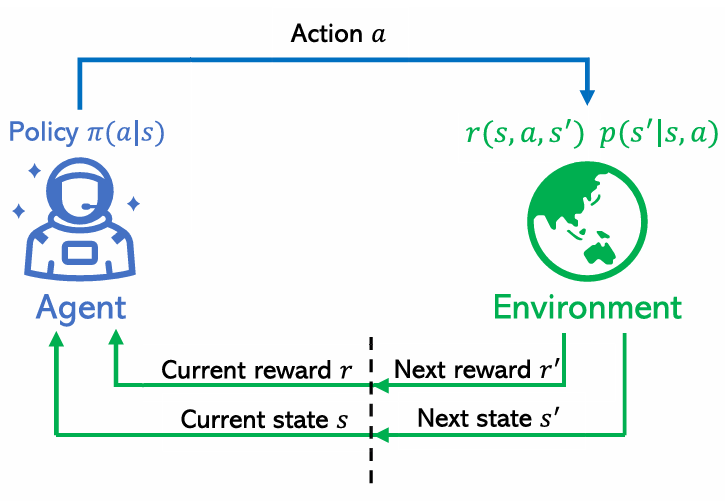
\includegraphics[width=0.5\linewidth]{Images/MDP_Diagram.png}
    \caption{Agent \DIFdelbeginFL \DIFdelFL{Interaction With }\DIFdelendFL \DIFaddbeginFL \DIFaddFL{interaction with an }\DIFaddendFL MDP\DIFaddbeginFL \DIFaddFL{.}\DIFaddendFL }
    \label{fig:MDP_Diagram}
\end{figure}

\subsection{Reinforcement Learning}\DIFdelbegin \DIFdel{RL is a decision-making computer program that starts without any prior knowledge , by learning through its own experiences of repeated random interactions }\DIFdelend \DIFaddbegin \label{sec:rl}
\DIFadd{In RL, an agent with no prior knowledge learns to make decisions from repeated interaction }\DIFaddend with an environment\DIFdelbegin \DIFdel{. It has the key benefit of being able to learn by exploring its training environment, and receiving feedback from this environment based on its actions \mbox{%DIFAUXCMD
\cite{LADOSZ20221}}\hskip0pt%DIFAUXCMD
. After training, the agent is graded on its performance with a different environment and then deployed.
}%DIFDELCMD < \newline
%DIFDELCMD < 

%DIFDELCMD < %%%
\DIFdel{Fundamentally, an RL }\DIFdelend \DIFaddbegin \DIFadd{, using the reward it receives as feedback \mbox{%DIFAUXCMD
\cite{LADOSZ20221}}\hskip0pt%DIFAUXCMD
. The }\DIFaddend problem is formalised as \DIFdelbegin \DIFdel{a Markov Decision Process (MDP ), as explained in Section~\ref{sec:MDP_ssSection} \mbox{%DIFAUXCMD
\cite{LADOSZ20221, DRL_Intrusion}}\hskip0pt%DIFAUXCMD
. The goal of the agent is to maximise the expected total reward defined by its reward function, by learning a policy}\DIFdelend \DIFaddbegin \DIFadd{an MDP (\mbox{%DIFAUXCMD
\cref{sec:MDP_ssSection}}\hskip0pt%DIFAUXCMD
) \mbox{%DIFAUXCMD
\cite{LADOSZ20221, DRL_Intrusion}}\hskip0pt%DIFAUXCMD
, and the agent learns a }\emph{\DIFadd{policy}}\DIFaddend : a probability distribution over actions $a_t$ \DIFdelbegin \DIFdel{for a given }\DIFdelend \DIFaddbegin \DIFadd{given the }\DIFaddend state $s_t$\DIFdelbegin \DIFdel{that makes the best decisions possible}\DIFdelend \DIFaddbegin \DIFadd{, chosen to maximise the expected total reward}\DIFaddend . RL methods fall into two main families. \textbf{Value-based} methods learn the expected return of each action and \DIFdelbegin \DIFdel{greedily }\DIFdelend \DIFaddbegin \DIFadd{typically }\DIFaddend choose the action with the highest estimate\DIFdelbegin \DIFdel{(typically)}\DIFdelend , while \textbf{policy-gradient} methods directly adjust the policy's parameters towards higher return \cite{williams1992reinforce}. \DIFdelbegin \DIFdel{Hybrid methods such as }\textbf{\DIFdel{actor-critic}} %DIFAUXCMD
\DIFdelend \DIFaddbegin \textbf{\DIFadd{Actor-critic}} \DIFadd{methods }\DIFaddend combine the two\DIFdelbegin \DIFdel{. A }\DIFdelend \DIFaddbegin \DIFadd{: a }\DIFaddend critic learns the expected return \DIFdelbegin \DIFdel{of each action, a value-based method}\DIFdelend \DIFaddbegin \DIFadd{from each state (a value function)}\DIFaddend , and an actor updates the policy using the critic's \DIFdelbegin \DIFdel{predictions, a policy-gradient method \mbox{%DIFAUXCMD
\cite{konda1999actorcritic}}\hskip0pt%DIFAUXCMD
.

}%DIFDELCMD < 

%DIFDELCMD < %%%
\DIFdel{The final goal of the agent is to maximise the sum of the rewards given from the environment. It makes decisions with a policy, a function that takes in a state and outputs the best possible action. There are two types of RL, policy approximation and value approximation. Policy approximation directly updates the policy function's parameters to make the best decisions - having to gradient descent to every action. Value function approximation introduces a value function to predict the downstream rewards of an action to simplify the policy update. Finally, }\DIFdelend \DIFaddbegin \DIFadd{estimates to judge whether an action was better or worse than expected \mbox{%DIFAUXCMD
\cite{konda1999actorcritic}}\hskip0pt%DIFAUXCMD
. PPO and A2C are both }\DIFaddend actor-critic \DIFdelbegin \DIFdel{combines the two}\DIFdelend \DIFaddbegin \DIFadd{methods}\DIFaddend .

%DIF >  =====================================================================
\section{Methodology}
\subsection{Problem Formulation}\DIFdelbegin \DIFdel{Consider the general problem we would like to research. There is some }\DIFdelend \DIFaddbegin \label{sec:problem}
\DIFadd{A }\DIFaddend cloud computing environment \DIFdelbegin \DIFdel{that }\DIFdelend receives a set of jobs \DIFdelbegin \DIFdel{according to some distribution that need to }\DIFdelend \DIFaddbegin \DIFadd{that must }\DIFaddend be assigned to a set of physical machines. Each job $j$ has a fixed processing duration $p_j$, a \DIFdelbegin \DIFdel{fixed }\DIFdelend multi-dimensional vector of \DIFdelbegin \DIFdel{its }\DIFdelend resource requirements $a_{jr}$ (\DIFdelbegin \DIFdel{e.g }\DIFdelend \DIFaddbegin \DIFadd{e.g.\ }\DIFaddend CPU, memory) which it occupies for \DIFdelbegin \DIFdel{the entire durationof its processing}\DIFdelend \DIFaddbegin \DIFadd{its entire duration}\DIFaddend , and a due date $d_j$ \DIFdelbegin \DIFdel{which the job should be completed by}\DIFdelend \DIFaddbegin \DIFadd{by which it should finish}\DIFaddend . Jobs are \DIFdelbegin \DIFdel{assumed to be }\DIFdelend independent of one another. \DIFdelbegin \DIFdel{To reflect that some jobs matter more than others, each job is given }\DIFdelend \DIFaddbegin \DIFadd{Each job has }\DIFaddend a priority weight $w_j$, \DIFdelbegin \DIFdel{which we can assume }\DIFdelend \DIFaddbegin \DIFadd{assumed }\DIFaddend to be set externally \DIFdelbegin \DIFdel{according to some business needs.
}%DIFDELCMD < \newline
%DIFDELCMD < 
%%%
\DIFdelend \DIFaddbegin \DIFadd{by business needs, to reflect that some jobs matter more than others.

}\DIFaddend 

Jobs are served by a set of identical machines \DIFdelbegin \DIFdel{, each limited only by }\DIFdelend \DIFaddbegin \DIFadd{$M$, each with }\DIFaddend a fixed capacity $C_r$ \DIFaddbegin \DIFadd{for every resource $r$}\DIFaddend . A machine may process several jobs \DIFdelbegin \DIFdel{simultaneously, provided the combined resource usage of every job }\DIFdelend \DIFaddbegin \DIFadd{at once, provided their combined usage }\DIFaddend does not exceed its capacity in any \DIFdelbegin \DIFdel{dimension. We model the scheduling to be }\DIFdelend \DIFaddbegin \DIFadd{resource. Scheduling is }\DIFaddend non-preemptive: each job is assigned to exactly one machine at a single start time \DIFdelbegin \DIFdel{, }\DIFdelend \DIFaddbegin \DIFadd{$s_j$ }\DIFaddend and runs uninterrupted until completion. \DIFdelbegin \DIFdel{We discretise time }\DIFdelend \DIFaddbegin \DIFadd{Time is divided }\DIFaddend into integer steps over a \DIFdelbegin \DIFdel{finite }\DIFdelend planning horizon $H$. The tardiness of \DIFdelbegin \DIFdel{a }\DIFdelend job $j$ is
\DIFdelbegin \DIFdel{then,
}\begin{displaymath}\DIFdel{%DIFDELCMD < \label{eq:tardiness}%%%

    T_j = \max\left(0,\; s_j + p_j - d_j\right).
}\end{displaymath}%DIFAUXCMD
\DIFdelend \DIFaddbegin \begin{equation}\DIFadd{\label{eq:tardiness}
    T_j = \max\left(0,\; s_j + p_j - d_j\right),
}\end{equation}\DIFaddend 
\DIFaddbegin \DIFadd{and $U_j = 1$ if job $j$ finishes late ($T_j > 0$), $0$ otherwise. }\DIFaddend Notation is summarised in Appendix~\ref{sec:AppendixA} \DIFdelbegin \DIFdel{, }\DIFdelend and the full constraint set in Appendix~\DIFdelbegin \DIFdel{\ref{} \textcolor{red}{ADD REFERENCE TO CONSTRAINT APPENDIX}

}\DIFdelend \DIFaddbegin \DIFadd{\ref{sec:AppendixB}.

}\DIFaddend 

\subsection{Objective \DIFdelbegin \DIFdel{Functions}%DIFDELCMD < \MBLOCKRIGHTBRACE
%DIFDELCMD < %%%
\DIFdel{The objective functions are the functions we would like to optimise for. In this project, two objective functions were used. The first (v1) weighs machine count (with machine activation $y_m$)}\DIFdelend \DIFaddbegin \DIFadd{Function}}\label{sec:objectives}
\DIFadd{The first objective tried weighted the number of machines used}\DIFaddend , weighted tardiness \DIFdelbegin \DIFdel{($w_jT_j$) }\DIFdelend and peak utilisation $\theta$\DIFdelbegin \DIFdel{with objective weights $\lambda$:
}\begin{displaymath}\DIFdel{%DIFDELCMD < \label{eq: Initial Objective Function}%%%

      \min \; \lambda_1 \sum_{m \in M} y_m \;+\; \lambda_2 \sum_{j \in J}
  w_j T_j \;+\; \lambda_3\, \theta,
  }\end{displaymath}%DIFAUXCMD
\DIFdelend \DIFaddbegin \DIFadd{:
}\begin{equation}\DIFadd{\label{eq:objective-v1}
    \min \; \lambda_1 \sum_{m \in M} y_m \;+\; \lambda_2 \sum_{j \in J} w_j T_j \;+\; \lambda_3\, \theta.
}\end{equation}\DIFaddend 
\DIFdelbegin \DIFdel{Experiments under v1 revealed that the training reward was inefficient with reward hacking \mbox{%DIFAUXCMD
\cite{skalse2022rewardhacking}}\hskip0pt%DIFAUXCMD
, and that unscheduled jobs incurred no loss. Essentially the objective could be optimised without considering tardiness. Moreover, the machine activation and hotspot penalties were found to be weak in that the activation penalty was an unnecessary once-off penalty, and the hotspot term inadvertently went against energy metrics and provides no real help to the RL agents. This term also opposes }\DIFdelend \DIFaddbegin \DIFadd{\mbox{%DIFAUXCMD
\Cref{eq:objective-v1} }\hskip0pt%DIFAUXCMD
could be gamed: unscheduled jobs cost nothing, so agents found high-reward schedules that left many jobs unassigned, a form of reward hacking \mbox{%DIFAUXCMD
\cite{skalse2022rewardhacking}}\hskip0pt%DIFAUXCMD
. Its peak-utilisation term also works against }\DIFaddend energy-efficient consolidation \cite{energyaware2012, fan2007powerprovisioning}. \DIFdelbegin \DIFdel{The revised objective (v2) is a sum of multiple metrics each weighted by $\lambda$:
}\begin{displaymath}\DIFdel{%DIFDELCMD < \label{eq:objective-v2}%%%

    \min \; J = \lambda_S \sum_{j} w_j T_j^{2}
              + \lambda_U \sum_{j} w_j U_j + \lambda_E E,
}\end{displaymath}%DIFAUXCMD
\DIFdelend \DIFaddbegin \DIFadd{It was replaced by a weighted sum of optional terms:
}\begin{equation}\DIFadd{\label{eq:objective-v2}
    \min \; J_{\lambda} = \underbrace{\sum_{j} w_j T_j^{2}}_{J}
          \;+\; \lambda_T \sum_{j} w_j T_j
          \;+\; \lambda_U \sum_{j} w_j U_j
          \;+\; \lambda_E E,
}\end{equation}\DIFaddend 
\DIFdelbegin \DIFdel{In order it covers squared tardiness($w_j T_j^{2}$), weighted late job count ($w_jU_j$}\DIFdelend \DIFaddbegin \DIFadd{covering squared tardiness, linear tardiness, the weighted number of late jobs (deadline violations}\DIFaddend ), and energy \DIFdelbegin \DIFdel{usage ($E)$. With this new objective , we can control which metrics we would like to examine for the project (by changing their weighted significance}\DIFdelend \DIFaddbegin \DIFadd{$E$, measured as total active machine-time \mbox{%DIFAUXCMD
\cite{fan2007powerprovisioning}}\hskip0pt%DIFAUXCMD
. The main objective of this project is $J$ alone ($\lambda_T = \lambda_U = \lambda_E = 0$}\DIFaddend ). Squared tardiness \DIFdelbegin \DIFdel{was included to incentivize choosing to have }\DIFdelend \DIFaddbegin \DIFadd{penalises a few very late jobs more than }\DIFaddend many slightly late \DIFdelbegin \DIFdel{jobs over having a few extremely late jobs . It also discourages never assigning a job , which v1 struggled with. }\DIFdelend \DIFaddbegin \DIFadd{ones, whereas linear tardiness can score very different schedules equally. $J$ is evaluated over an }\emph{\DIFadd{extended horizon}}\DIFadd{: jobs are released only within $[0, H)$, but no job is ever discarded, and an unfinished job keeps accumulating tardiness until it completes. Leaving a job unscheduled is therefore always costly, which removes the loophole in \mbox{%DIFAUXCMD
\cref{eq:objective-v1}}\hskip0pt%DIFAUXCMD
. The other terms are switched on only in the multi-objective experiments (\mbox{%DIFAUXCMD
\cref{sec:mo-method}}\hskip0pt%DIFAUXCMD
).

}\DIFaddend 

\subsection{Offline and Online Cases}\DIFdelbegin \DIFdel{We would like to study two }\DIFdelend \DIFaddbegin \label{sec:cases}
\DIFadd{Two }\DIFaddend cases of the problem \DIFdelbegin \DIFdel{: offline when }\DIFdelend \DIFaddbegin \DIFadd{are studied. In the }\textbf{\DIFadd{offline}} \DIFadd{case }\DIFaddend all jobs are known and available at \DIFdelbegin \DIFdel{$t=0$ but only a single }\DIFdelend \DIFaddbegin \DIFadd{$t = 0$, and at most one }\DIFaddend job can be \DIFdelbegin \DIFdel{assigned at each time index, and an online case where }\DIFdelend \DIFaddbegin \DIFadd{started per time step. In the }\textbf{\DIFadd{online}} \DIFadd{case }\DIFaddend jobs arrive (\DIFaddbegin \DIFadd{are }\DIFaddend revealed) over time \DIFdelbegin \DIFdel{through }\DIFdelend \DIFaddbegin \DIFadd{according to }\DIFaddend a Poisson process \cite{kleinrock1975queueing, mao2016deeprm}\DIFdelbegin \DIFdel{but multiple jobs can be assigned at any given timestep.

}%DIFDELCMD < \newline
%DIFDELCMD < %%%
\DIFdel{The difficulty for }\DIFdelend \DIFaddbegin \DIFadd{, and any number of jobs may be started at the same time step.

}

\DIFadd{The difficulty of }\DIFaddend the online case \DIFdelbegin \DIFdel{of the random job arrivals }\DIFdelend is set by the load factor \DIFdelbegin \begin{displaymath}\DIFdel{%DIFDELCMD < \label{eq:rho}%%%

    \rho = \max_{r \in R} \frac{\nu\, \mathbb{E}[p_j a_{jr}]}{|M|\, C_r},
}\end{displaymath}%DIFAUXCMD
\DIFdelend \DIFaddbegin \DIFadd{$\rho$, which measures how busy the cluster is on average. A job $j$ brings $p_j a_{jr}$ units of work for resource $r$ (resource units multiplied by time steps). If jobs arrive at rate $\nu$ per time step, on average $\nu\,\mathbb{E}[p_j a_{jr}]$ units of work arrive per time step, while the cluster can process at most $|M|\, C_r$ units per time step. Their ratio is the standard utilisation of a queueing system \mbox{%DIFAUXCMD
\cite{kleinrock1975queueing}}\hskip0pt%DIFAUXCMD
, and taking the largest ratio over resources picks out the bottleneck resource:
}\begin{equation}\DIFadd{\label{eq:rho}
    \rho = \max_{r \in R} \frac{\nu\, \mathbb{E}[p_j a_{jr}]}{|M|\, C_r}.
}\end{equation}\DIFaddend 
\DIFdelbegin \DIFdel{where }\DIFdelend \DIFaddbegin \DIFadd{For $\rho < 1$ the cluster can keep up on average; for $\rho \ge 1$ work arrives faster than it can be processed and the queue necessarily grows. For each target load, the arrival rate }\DIFaddend $\nu$ \DIFdelbegin \DIFdel{is the arrival rate. Work accumulates when $\rho\ge1$. }\DIFdelend \DIFaddbegin \DIFadd{is chosen to give that $\rho$. }\DIFaddend Loads from $\rho = 0.50$ to $1.10$ are studied\DIFdelbegin \DIFdel{, with log-normal job sizes matching the right-skewed distributions of real cluster traces \mbox{%DIFAUXCMD
\cite{reiss2012googletrace, cortez2017resourcecentral}}\hskip0pt%DIFAUXCMD
}\DIFdelend .

\subsection{Markov Decision Process}\DIFaddbegin \label{sec:mdp}
\DIFaddend To formulate this problem for our algorithms \DIFdelbegin \DIFdel{, we use a Markov Decision Process $(S,A,P,R,\gamma)$ as discussed in section ~\ref{sec:MDP_ssSection}.

}%DIFDELCMD < \newline
%DIFDELCMD < 
%%%
\DIFdelend \DIFaddbegin \DIFadd{we use an MDP $(S, A, P, R, \gamma)$ as described in \mbox{%DIFAUXCMD
\cref{sec:MDP_ssSection}}\hskip0pt%DIFAUXCMD
.

}\DIFaddend 

\paragraph{State $S$\DIFaddbegin \DIFadd{.}\DIFaddend } \DIFdelbegin \DIFdel{. We define the state to hold each currently waiting job 's ($j\in J_t\subseteq J$) features $F_j=(p_j, A_j, d_j, w_j)$, along with each currently processing job where a job enters }\DIFdelend \DIFaddbegin \DIFadd{The state holds the features $F_j = (p_j, a_j, d_j, w_j)$ of each waiting job $j \in J_t \subseteq J$, and, for each job in }\DIFaddend the processing set \DIFdelbegin \DIFdel{$P_t\subseteq J$ when it gets assigned. For each processing job, we instead hold $G_j=(m_j,s_j,p_j)$ that includes which machine the job is assigned to, its }\DIFdelend \DIFaddbegin \DIFadd{$P_t \subseteq J$ (jobs that have started and not finished), $G_j = (m_j, s_j, p_j)$: its machine, }\DIFaddend start time and \DIFdelbegin \DIFdel{total duration. On top of the jobs, we include include the }\DIFdelend \DIFaddbegin \DIFadd{duration. It also holds the }\DIFaddend remaining capacity of each machine,
\begin{equation}\label{eq:remaining-capacity}
    R_{mrt} = C_r - \sum_{j \in P_t:\ m_j = m} a_{jr},
\end{equation}
and \DIFdelbegin \DIFdel{$y=(y_m)_{m\in M}$ to record }\DIFdelend \DIFaddbegin \DIFadd{$y = (y_m)_{m \in M}$, recording }\DIFaddend which machines are \DIFdelbegin \DIFdel{online. This yields a state
vector,
}\DIFdelend \DIFaddbegin \DIFadd{switched on. This gives the state
}\DIFaddend \begin{equation}\label{eq:state}
    s_t = \big(J_t,\ P_t,\ \{F_j\}_{j \in J_t},\ \{G_j\}_{j \in P_t},\ \{R_{mrt}\}_{m \in M,\, r \in R},\ y,\ t\big).
\end{equation}
\DIFdelbegin \paragraph{\DIFdel{Action Space $A$}}%DIFAUXCMD
\addtocounter{paragraph}{-1}%DIFAUXCMD
\DIFdel{.

}\DIFdelend \DIFaddbegin \DIFadd{The agent also sees each machine's free capacity over the next few time steps, computed from $G_j$ (no new information, but easier to learn from).

}

\paragraph{\DIFadd{Action space $A$.}} \DIFaddend At each step, the agent can \DIFdelbegin \DIFdel{take actions of assigning waiting jobs to machines, and/or idling,
}\begin{displaymath}\DIFdel{%DIFDELCMD < \label{eq:action-flat}%%%

    \mathcal{A}_t = \{(j, m) : j \in J_t,\ m \in M\} \cup \{\text{idle}\}.
}\end{displaymath}%DIFAUXCMD
\DIFdelend \DIFaddbegin \DIFadd{assign a waiting job to a machine, or idle:
}\begin{equation}\DIFadd{\label{eq:action-flat}
    A_t = \{(j, m) : j \in J_t,\ m \in M\} \cup \{\text{idle}\}.
}\end{equation}\DIFaddend 
\DIFdelbegin \DIFdel{For the offline case, an agent can only produce a single action at each time step. For the onlinecase, an agent can continuously do actions at the same step$t$, only progressing to the next time step when it decides to idle}\DIFdelend \DIFaddbegin \DIFadd{Assignments that would exceed a machine's capacity are masked out \mbox{%DIFAUXCMD
\cite{huang2020invalidmasking}}\hskip0pt%DIFAUXCMD
. Offline, each assignment is followed by a time step; online, the agent may make several assignments per time step, and time advances only when it idles. Idling is always allowed: deliberately leaving capacity free for later jobs is a behaviour RL could learn, and schedules that never idle can exclude the optimum \mbox{%DIFAUXCMD
\cite{giffler1960active}}\hskip0pt%DIFAUXCMD
. An idle advances time to the next job arrival or completion, so the agent cannot idle forever}\DIFaddend .

\paragraph{Transition dynamics $P$.} \DIFdelbegin \DIFdel{Briefly, an assignment action }\DIFdelend \DIFaddbegin \DIFadd{An assignment }\DIFaddend $(j, m)$ moves job $j$ from $J_t$ to $P_t$ with $s_j = t$ and $m_j = m$, \DIFdelbegin \DIFdel{activating }\DIFdelend \DIFaddbegin \DIFadd{switching }\DIFaddend machine $m$ \DIFaddbegin \DIFadd{on }\DIFaddend if needed. When time advances\DIFdelbegin \DIFdel{(after every action for offline, and only after idle for online), }\DIFdelend \DIFaddbegin \DIFadd{, }\DIFaddend completed jobs leave the processing set by \cref{eq:processing-update} \DIFdelbegin \DIFdel{, their capacityis released, and }\DIFdelend \DIFaddbegin \DIFadd{and release their capacity; }\DIFaddend online, newly arrived jobs join $J_{t+1}$. Transitions are deterministic \DIFdelbegin \DIFdel{for offlineand stochastic for }\DIFdelend \DIFaddbegin \DIFadd{offline, and random }\DIFaddend online only through \DIFdelbegin \DIFdel{arrivals.
}\begin{displaymath}\DIFdel{%DIFDELCMD < \label{eq:processing-update}%%%

    P_{t+1} = \{k \in P_t : s_k + p_k > t + 1\},
}\end{displaymath}%DIFAUXCMD
\DIFdelend \DIFaddbegin \DIFadd{the arrivals.
}\begin{equation}\DIFadd{\label{eq:processing-update}
    P_{t+1} = \{k \in P_t : s_k + p_k > t + 1\}.
}\end{equation}\DIFaddend 

\paragraph{Reward $R$.} \DIFdelbegin \DIFdel{This project used both v1 and v2 rewards where stated in later sections (\mbox{%DIFAUXCMD
\cref{sec:objectives}}\hskip0pt%DIFAUXCMD
).

}\DIFdelend \DIFaddbegin \DIFadd{The reward is the negative of the objective, charged as it accrues: a late job of weight $w_j$ is charged $w_j(2k+1)$ in its $k$-th late time step, and since $\sum_{k=0}^{T_j-1}(2k+1) = T_j^2$ the charges add up to exactly $w_j T_j^2$. Maximising total reward is therefore the same as minimising $J$ in \mbox{%DIFAUXCMD
\cref{eq:objective-v2}}\hskip0pt%DIFAUXCMD
. To give the agent earlier feedback, a potential-based shaping term is added, which provably leaves the optimal policy unchanged \mbox{%DIFAUXCMD
\cite{ng1999shaping}}\hskip0pt%DIFAUXCMD
.

}\DIFaddend 

\DIFdelbegin 
%DIFAUXCMD
\addtocounter{subsection}{-1}%DIFAUXCMD
\DIFdel{In this project, a variety of algorithms are examined, grouped into four categories. We summarise these algorithms as follows. }%DIFDELCMD < 

%DIFDELCMD < %%%

%DIFAUXCMD
\addtocounter{subsubsection}{-1}%DIFAUXCMD
\paragraph{\DIFdel{Reinforcement Learning.}} %DIFAUXCMD
\addtocounter{paragraph}{-1}%DIFAUXCMD
\DIFdel{All RL policy methods examined are actor-critic methods: A2C and PPO for their robustness and simplicity. We consider these algorithms under several action-space designs }\DIFdelend \DIFaddbegin \paragraph{\DIFadd{Action-space designs.}} \DIFadd{The full action space \mbox{%DIFAUXCMD
\cref{eq:action-flat} }\hskip0pt%DIFAUXCMD
has 1001 actions for 100 jobs and 10 machines. Large discrete action spaces are a known difficulty for policy-gradient methods \mbox{%DIFAUXCMD
\cite{dulacarnold2015largeactionspaces}}\hskip0pt%DIFAUXCMD
, while successful prior schedulers use far fewer actions \mbox{%DIFAUXCMD
\cite{mao2016deeprm, mao2019decima}}\hskip0pt%DIFAUXCMD
. Six designs were therefore compared}\DIFaddend :
\begin{itemize}
    \item \textbf{Option 0 -- Direct \DIFdelbegin \DIFdel{Job-Machine Selection:}\DIFdelend \DIFaddbegin \DIFadd{job-machine selection.}\DIFaddend } The policy picks a (job, machine) pair \DIFdelbegin \DIFdel{with a flat network or }\DIFdelend \DIFaddbegin \DIFadd{from \mbox{%DIFAUXCMD
\cref{eq:action-flat}}\hskip0pt%DIFAUXCMD
, using a }\DIFaddend pointer-network architecture \cite{vinyals2015pointernet, kool2019attention}.
    \DIFdelbegin \DIFdel{A large discrete action space is a known struggle with policy-gradient methods.
    }\DIFdelend \item \textbf{Option 1 -- \DIFdelbegin \DIFdel{Hyper-heuristic }\DIFdelend Rule \DIFdelbegin \DIFdel{Selection:}\DIFdelend \DIFaddbegin \DIFadd{selection.}\DIFaddend } \DIFdelbegin \DIFdel{The }\DIFdelend \DIFaddbegin \DIFadd{At each decision the }\DIFaddend policy chooses which dispatching rule to apply\DIFdelbegin \DIFdel{at each decision \mbox{%DIFAUXCMD
\cite{burke2013hyperheuristicsurvey, lassoued2026hyperheuristic}}\hskip0pt%DIFAUXCMD
}\DIFdelend \DIFaddbegin \DIFadd{: one of seven priority rules, each with First-Fit or Consolidate placement (\mbox{%DIFAUXCMD
\cref{sec:baselines}}\hskip0pt%DIFAUXCMD
), making the agent a selection hyper-heuristic \mbox{%DIFAUXCMD
\cite{burke2013hyperheuristicsurvey, lassoued2026hyperheuristic}}\hskip0pt%DIFAUXCMD
.
    }\DIFaddend \item \textbf{Option 2 -- Priority \DIFdelbegin \DIFdel{Learning:}\DIFdelend \DIFaddbegin \DIFadd{learning.}\DIFaddend } The policy \DIFdelbegin \DIFdel{scores jobs directly with either learned or directly engineered features, }\DIFdelend \DIFaddbegin \DIFadd{picks which waiting job to start next, learning its own priority from the raw job features; the chosen job is then placed by the First-Fit rule. This is }\DIFaddend a hybrid of RL \DIFaddbegin \DIFadd{and a dispatching heuristic: RL learns the ordering, a fixed rule does the placement \mbox{%DIFAUXCMD
\cite{mao2016deeprm, min2022atctuning}}\hskip0pt%DIFAUXCMD
}\DIFaddend .
    \item \textbf{Option 3 -- \DIFdelbegin \DIFdel{Windowed }\DIFdelend Priority \DIFdelbegin \DIFdel{:}\DIFdelend \DIFaddbegin \DIFadd{learning with an ATC feature.}\DIFaddend } Option 2 \DIFdelbegin \DIFdel{, but masked to only }\DIFdelend \DIFaddbegin \DIFadd{with the Apparent Tardiness Cost index \mbox{%DIFAUXCMD
\cite{vepsalainen1987atc} }\hskip0pt%DIFAUXCMD
added as an extra job feature. Option 3w is the same, restricted to }\DIFaddend the 20 most urgent jobs \cite{mao2016deeprm}\DIFaddbegin \DIFadd{.
    }\DIFaddend \item \textbf{Option 4 -- Action \DIFdelbegin \DIFdel{Branching:}\DIFdelend \DIFaddbegin \DIFadd{branching.}\DIFaddend } \DIFdelbegin \DIFdel{Job and }\DIFdelend \DIFaddbegin \DIFadd{The job and the }\DIFaddend machine are chosen by two separate \DIFaddbegin \DIFadd{network }\DIFaddend heads instead of \DIFdelbegin \DIFdel{together (flat) \mbox{%DIFAUXCMD
\cite{tavakoli2018actionbranching}}\hskip0pt%DIFAUXCMD
}\DIFdelend \DIFaddbegin \DIFadd{one joint action \mbox{%DIFAUXCMD
\cite{tavakoli2018actionbranching}}\hskip0pt%DIFAUXCMD
.
}\DIFaddend \end{itemize}

\DIFdelbegin \DIFdel{Moreover, variants of the two RL algorithms: Reward Constrained Policy Optimisation }\DIFdelend \DIFaddbegin 

\subsection{\DIFadd{Learning Algorithms}}\label{sec:algorithms}
\DIFadd{All RL agents use PPO \mbox{%DIFAUXCMD
\cite{schulman2017ppo} }\hskip0pt%DIFAUXCMD
or A2C \mbox{%DIFAUXCMD
\cite{mnih2016a3c}}\hskip0pt%DIFAUXCMD
, as implemented in Stable-Baselines3 \mbox{%DIFAUXCMD
\cite{raffin2021sb3}}\hskip0pt%DIFAUXCMD
. Both are actor-critic methods (\mbox{%DIFAUXCMD
\cref{sec:rl}}\hskip0pt%DIFAUXCMD
). PPO limits how far the policy can change in a single update, which makes training more stable; A2C uses simpler, more frequent updates. Both are widely used and comparable within one framework \mbox{%DIFAUXCMD
\cite{huang2022a2cppo}}\hskip0pt%DIFAUXCMD
.

}

\paragraph{\DIFadd{Approaches tried before the final setup.}} \DIFadd{The final setup was reached through several rounds of training, diagnosis and revision. Alternatives tried along the way included reward-constrained policy optimisation }\DIFaddend (RCPO) \DIFdelbegin \DIFdel{for a different reward function approach, and PPO-Lagrangian were also examined. }\DIFdelend \DIFaddbegin \DIFadd{\mbox{%DIFAUXCMD
\cite{tessler2019rcpo} }\hskip0pt%DIFAUXCMD
and PPO-Lagrangian \mbox{%DIFAUXCMD
\cite{stooke2020pidlagrangian}}\hskip0pt%DIFAUXCMD
, which treat tardiness as a constraint rather than a cost, dense and shaped tardiness rewards, curriculum learning, and a version in which idling was forbidden whenever a job could be placed. Under the original objective (\mbox{%DIFAUXCMD
\cref{eq:objective-v1}}\hskip0pt%DIFAUXCMD
), none of these produced an agent that beat the best heuristic on tardiness. The final version fixed two faults in the previous one: the critic never learned, because squared-tardiness rewards are very large, and a deterministic policy could idle forever. These were fixed by reward scaling \mbox{%DIFAUXCMD
\cite{engstrom2020implementation, andrychowicz2021onpolicy}}\hskip0pt%DIFAUXCMD
, event-driven idling (\mbox{%DIFAUXCMD
\cref{sec:mdp}}\hskip0pt%DIFAUXCMD
) and a two-stage evaluation rule (\mbox{%DIFAUXCMD
\cref{sec:evaluation}}\hskip0pt%DIFAUXCMD
). In addition, the critic (but not the policy) sees a summary of jobs that have not arrived yet, which reduces noise in online training without biasing the policy \mbox{%DIFAUXCMD
\cite{mao2019variance, pinto2018asymmetric}}\hskip0pt%DIFAUXCMD
. Appendix~\ref{sec:AppendixD} gives the diagnosis.

}\DIFaddend 

\DIFdelbegin 
%DIFAUXCMD
\addtocounter{subsubsection}{-1}%DIFAUXCMD
\paragraph{\DIFdel{Dispatching Heuristics}}%DIFAUXCMD
\addtocounter{paragraph}{-1}%DIFAUXCMD
\DIFdel{. }\DIFdelend \DIFaddbegin \subsection{\DIFadd{Methods Compared}}\label{sec:baselines}
\paragraph{\DIFadd{Dispatching heuristics.}} \DIFaddend Each heuristic combines a priority rule\DIFdelbegin \DIFdel{to choose }\DIFdelend \DIFaddbegin \DIFadd{, which chooses }\DIFaddend the next job, \DIFdelbegin \DIFdel{and }\DIFdelend \DIFaddbegin \DIFadd{with }\DIFaddend a placement rule\DIFdelbegin \DIFdel{to choose the next machine }\DIFdelend \DIFaddbegin \DIFadd{, which chooses its machine \mbox{%DIFAUXCMD
\cite{pinedo2016scheduling}}\hskip0pt%DIFAUXCMD
}\DIFaddend .
\begin{itemize}
    \item \textbf{Priority \DIFdelbegin \DIFdel{Rules}\DIFdelend \DIFaddbegin \DIFadd{rules}\DIFaddend :} Earliest Deadline First (EDF) and Least Slack Time (LST), which prioritise urgency \DIFaddbegin \DIFadd{\mbox{%DIFAUXCMD
\cite{pinedo2016scheduling}}\hskip0pt%DIFAUXCMD
}\DIFaddend ; Shortest and Longest Processing Time (SPT\DIFdelbegin \DIFdel{) and (LPT) }\DIFdelend \DIFaddbegin \DIFadd{, LPT) \mbox{%DIFAUXCMD
\cite{pinedo2016scheduling, graham1969lpt}}\hskip0pt%DIFAUXCMD
}\DIFaddend ; Weighted SPT (WSPT) \DIFaddbegin \DIFadd{\mbox{%DIFAUXCMD
\cite{smith1956wspt}}\hskip0pt%DIFAUXCMD
}\DIFaddend ; First-Come-First-Served (FCFS\DIFdelbegin \DIFdel{), and the }\DIFdelend \DIFaddbegin \DIFadd{, also known as First-In-First-Out, FIFO); }\DIFaddend Apparent Tardiness Cost (ATC)\DIFdelbegin \DIFdel{rule, balancing }\DIFdelend \DIFaddbegin \DIFadd{, which balances }\DIFaddend job weight, length and urgency \DIFdelbegin \DIFdel{.
    }\DIFdelend \DIFaddbegin \DIFadd{\mbox{%DIFAUXCMD
\cite{vepsalainen1987atc}}\hskip0pt%DIFAUXCMD
; and the weighted-tardiness rules WMDD \mbox{%DIFAUXCMD
\cite{kanet2004wmdd} }\hskip0pt%DIFAUXCMD
and COVERT \mbox{%DIFAUXCMD
\cite{carroll1965covert}}\hskip0pt%DIFAUXCMD
. Because the published weighted rules performed poorly under squared tardiness, three weighted variants were constructed for this project: weighted LST (WLST) and weighted EDF (WEDF), which scale a job's slack by its weight, and Marginal Delay Cost (MDC), which applies Smith's ratio rule \mbox{%DIFAUXCMD
\cite{smith1956wspt} }\hskip0pt%DIFAUXCMD
to the marginal increase in squared tardiness. These were added after the first RL results were seen.
    }\DIFaddend \item \textbf{Placement \DIFdelbegin \DIFdel{Rules}\DIFdelend \DIFaddbegin \DIFadd{rules}\DIFaddend :} First-Fit, Best-Fit \DIFdelbegin \DIFdel{, }\DIFdelend \DIFaddbegin \DIFadd{and }\DIFaddend Worst-Fit \DIFaddbegin \DIFadd{\mbox{%DIFAUXCMD
\cite{johnson1973binpacking}}\hskip0pt%DIFAUXCMD
}\DIFaddend , and Consolidate, \DIFdelbegin \DIFdel{a more energy aware approach \mbox{%DIFAUXCMD
\cite{energyaware2012}}\hskip0pt%DIFAUXCMD
}\DIFdelend \DIFaddbegin \DIFadd{an energy-aware rule that prefers machines that are already on \mbox{%DIFAUXCMD
\cite{energyaware2012}}\hskip0pt%DIFAUXCMD
.
    }\DIFaddend \item \textbf{Tetris:} \DIFdelbegin \DIFdel{A }\DIFdelend \DIFaddbegin \DIFadd{a }\DIFaddend multi-resource packing heuristic \DIFdelbegin \DIFdel{scoring }\DIFdelend \DIFaddbegin \DIFadd{that scores }\DIFaddend job-machine pairs jointly \DIFaddbegin \DIFadd{\mbox{%DIFAUXCMD
\cite{grandl2014tetris}}\hskip0pt%DIFAUXCMD
}\DIFaddend .
\end{itemize}

\DIFdelbegin \paragraph{\DIFdel{Metaheuristic:}}
%DIFAUXCMD
\addtocounter{paragraph}{-1}%DIFAUXCMD
%DIFDELCMD < \begin{itemize}
%DIFDELCMD <     \item %%%
\textbf{\DIFdel{Particle Swarm Optimisation (PSO)}}%DIFAUXCMD
\DIFdel{.

Each }\DIFdelend \DIFaddbegin \DIFadd{In total, the twelve priority rules and four placement rules give 48 heuristics, plus Tetris; random rule choice is included as a sanity check.

}

\paragraph{\DIFadd{Metaheuristic.}} \DIFadd{Particle Swarm Optimisation (PSO) \mbox{%DIFAUXCMD
\cite{kennedy1995pso}}\hskip0pt%DIFAUXCMD
, in which each }\DIFaddend particle encodes a job \DIFdelbegin \DIFdel{and machine ordering which is decoded with }\DIFdelend \DIFaddbegin \DIFadd{ordering that }\DIFaddend a placement rule \DIFaddbegin \DIFadd{decodes }\DIFaddend into a schedule\DIFdelbegin \DIFdel{. 
}%DIFDELCMD < \end{itemize}
%DIFDELCMD < 
%%%
\DIFdelend \DIFaddbegin \DIFadd{, was evaluated in earlier rounds of the project. It was worse than the best dispatching rule in every setting tested, so it is not part of the final comparison.

}\DIFaddend 

\DIFdelbegin \paragraph{\DIFdel{Exact Solver:}}
%DIFAUXCMD
\addtocounter{paragraph}{-1}%DIFAUXCMD
%DIFDELCMD < \begin{itemize}
%DIFDELCMD <     \item %%%
\textbf{\DIFdel{CP-SAT}}%DIFAUXCMD
\DIFdel{.

Constraint programming which models the scheduling problem and environment exactly}\DIFdelend \DIFaddbegin \paragraph{\DIFadd{Exact solver.}} \DIFadd{CP-SAT \mbox{%DIFAUXCMD
\cite{ortools}}\hskip0pt%DIFAUXCMD
, a constraint-programming solver, models the problem of Appendix~\ref{sec:AppendixB} exactly. Within a time limit it returns the best schedule it has found, whose $J$ is an upper bound on the optimum}\DIFaddend , \DIFdelbegin \DIFdel{finding the proven optimumschedule if given enough time, otherwise a }\DIFdelend \DIFaddbegin \DIFadd{together with a proven }\DIFaddend lower bound on the optimum. \DIFdelbegin %DIFDELCMD < \end{itemize}
%DIFDELCMD < 
%%%
\DIFdelend \DIFaddbegin \DIFadd{When the two meet, the schedule is proven optimal. CP-SAT was given 60 seconds per instance.

}\DIFaddend 

\subsection{Implementation}\DIFaddbegin \label{sec:implementation}
\DIFaddend The environment, agents and evaluation pipeline are implemented in Python\footnote{\url{https://github.com/Ethan-Ty-Riekert/Neural-Knapsack-Research-Project}} using Gymnasium and Stable-Baselines3 \cite{raffin2021sb3}. The \DIFdelbegin \DIFdel{original environment and mathematical formulation implementation into code was done manually, with all model implementations}\DIFdelend \DIFaddbegin \DIFadd{environment and the translation of the mathematical formulation into code were written by hand; model implementation}\DIFaddend , training and evaluation \DIFdelbegin \DIFdel{done with }\DIFdelend \DIFaddbegin \DIFadd{were done with the help of }\DIFaddend Claude Code (\DIFdelbegin \DIFdel{Anthropic)to allow for fast code iteration and implementation.

}%DIFDELCMD < \begin{itemize}

%DIFDELCMD <     \item %%%

\textbf{\DIFdel{Context. }}%DIFAUXCMD
\DIFdel{Claude is provided with the latest version of the current research report, formulations, and experimental logs
    }%DIFDELCMD < \item %%%

\textbf{\DIFdel{Rules. }}%DIFAUXCMD
\DIFdel{A fixed set of rules for Claude to follow: Every design decision has to be cited and justified, or derived. Implementation, research and discussions have to remain mathematical grounded
    }%DIFDELCMD < \item %%%

\textbf{\DIFdel{Benchmarking and Results. }}%DIFAUXCMD
\DIFdel{All results and benchmarks are run autonomously by Claude with a constant queue, ready for personal review.
    }%DIFDELCMD < \item %%%

\textbf{\DIFdel{Diagnostics and Research. }}%DIFAUXCMD
\DIFdel{Unexpected results and failures are investigated and checked against literature
    }%DIFDELCMD < \item %%%

\textbf{\DIFdel{Recording and Revisions. }}%DIFAUXCMD
\DIFdel{Every decision and result is to be recorded in an experiment log
}

%DIFDELCMD < \end{itemize}
%DIFDELCMD < %%%
\DIFdel{All modeling decisions and formulations are reviewed and approved personally. Using Claude as a coding assistant allowed for far more experiments to be run and analysed, along with constant model improvements and iterations than would otherwise have been possible independently. It also allowed for easier discussions of modelling decisions against other papers. Moreover, weekly optimisation, mathematical rigour, and factual scans were done with separate Claude agents to ensure correctness.

}\DIFdelend \DIFaddbegin \DIFadd{see the Generative AI Use Statement).

}\DIFaddend 

\DIFdelbegin 
%DIFAUXCMD
\addtocounter{subsubsection}{-1}%DIFAUXCMD
\DIFdelend \DIFaddbegin \subsection{\DIFadd{Experimental Setup}}\label{sec:setup}
\DIFaddend \paragraph{\DIFdelbegin \DIFdel{Offline}\DIFdelend \DIFaddbegin \DIFadd{Instances.}\DIFaddend } \DIFaddbegin \DIFadd{Offline }\DIFaddend instances have 100 jobs, 10 machines \DIFdelbegin \DIFdel{, }\DIFdelend \DIFaddbegin \DIFadd{and }\DIFaddend 4 resources with \DIFdelbegin \DIFdel{$C_r=30$, $H=100$}\DIFdelend \DIFaddbegin \DIFadd{$C_r = 30$, and $H = 100$}\DIFaddend . Job durations and \DIFaddbegin \DIFadd{resource }\DIFaddend demands are drawn uniformly from \DIFdelbegin \DIFdel{$\{1,\dots,9\}$, and job weights $\{1,\dots,5\}$, with deadlines of medium tightness ($\mathrm{TF} = 0.5$)\mbox{%DIFAUXCMD
\cite{potts1985wtardiness}}\hskip0pt%DIFAUXCMD
. A matching preset with all $w_j = 1$ is generated to isolate the effects of considering weights. }%DIFDELCMD < 

%DIFDELCMD < %%%
\paragraph{\DIFdel{Online}} %DIFAUXCMD
\addtocounter{paragraph}{-1}%DIFAUXCMD
\DIFdel{instances use the same setup with addition of Poisson arrivals over $[0, H)$ at loads $\rho\in\{0.50, 0.75, 0.95, 1.10\}$ and deadline slack drawn between 10 }\DIFdelend \DIFaddbegin \DIFadd{$\{1, \dots, 9\}$, and weights from $\{1, \dots, 5\}$. Deadline tightness is set by the tardiness factor TF \mbox{%DIFAUXCMD
\cite{potts1985wtardiness}}\hskip0pt%DIFAUXCMD
: larger TF means tighter deadlines on average. The main setting uses TF $= 0.5$ (medium), with 0.2 }\DIFaddend and \DIFdelbegin \DIFdel{60. Moreover job resource }\DIFdelend \DIFaddbegin \DIFadd{0.8 as loose and tight variants. A unit-weight setting ($w_j = 1$) isolates the effect of job weights. Online instances always use weighted jobs (there is no unit-weight online setting) and add Poisson arrivals at loads $\rho \in \{0.50, 0.75, 0.95, 1.10\}$; each job's deadline is its arrival time plus a random slack, the online counterpart of TF. Online job }\DIFaddend sizes are log-normal \DIFdelbegin \DIFdel{, mean-matched to the offline distribution. }\DIFdelend \DIFaddbegin \DIFadd{(right-skewed, like real cluster traces \mbox{%DIFAUXCMD
\cite{reiss2012googletrace, cortez2017resourcecentral}}\hskip0pt%DIFAUXCMD
). Because every RL study takes hours to days of compute, RL agents were trained and evaluated in one offline setting (TF $= 0.5$, with weighted and unit weights) and one online setting ($\rho = 0.95$: heavy load, but below saturation, so scheduling decisions matter most). The other loads and deadline tightnesses were run for the heuristics only. Appendix~\ref{sec:AppendixD} gives the exact distributions.

}\DIFaddend 

\DIFdelbegin \paragraph{\DIFdel{Training}}%DIFAUXCMD
\addtocounter{paragraph}{-1}%DIFAUXCMD
\DIFdel{. }\DIFdelend \DIFaddbegin \paragraph{\DIFadd{Training and tuning.}} \DIFaddend An agent learns \DIFdelbegin \DIFdel{by interacting with an environment over a sequence of episodes. One episode is one complete problem instance, i.e an instance of making decisions until the horizon $H$ is reached for some given environment. Every episode uses a newly generated random instanceof job parameters so that the agent never sees }\DIFdelend \DIFaddbegin \DIFadd{over episodes, each a complete, newly generated problem instance, so it never trains on }\DIFaddend the same problem twice\DIFdelbegin \DIFdel{and can thereby generalise. Every RL action design was trained with PPO and A2C, }\DIFdelend \DIFaddbegin \DIFadd{. Training, validation (20 instances) and test (50 instances) use disjoint random seeds, so test instances are never seen in training or tuning. Every combination of design (6), algorithm (2) and case (2) had its own hyperparameter search, 24 studies in all, run }\DIFaddend with the same \DIFdelbegin \DIFdel{tuning and training budgets. Hyperparameters were tuned with Optuna \mbox{%DIFAUXCMD
\cite{akiba2019optuna} }\hskip0pt%DIFAUXCMD
using }\DIFdelend \DIFaddbegin \DIFadd{protocol: Optuna \mbox{%DIFAUXCMD
\cite{akiba2019optuna} }\hskip0pt%DIFAUXCMD
with }\DIFaddend the TPE sampler \cite{bergstra2011tpe}\DIFdelbegin \DIFdel{and median pruning. 20 trials of 100}\DIFdelend , \DIFaddbegin \DIFadd{12 trials of 300,}\DIFaddend 000 steps\DIFdelbegin \DIFdel{for each model design, algorithm and case (offline and online) were put into the Optuna search. Every 25, 000 steps, each trialwas evaluated against 5 validation instances and stopped early if it was worse than }\DIFdelend \DIFaddbegin \DIFadd{, }\DIFaddend the \DIFaddbegin \DIFadd{first trial always being the library defaults. Poor trials were stopped early by median pruning, which compares a trial's validation $J$ with the }\DIFaddend median of earlier trials \DIFdelbegin \DIFdel{. The best configurationof hyperparameters is then trained for 300, 000 steps across 4 parallel environments. Because RL deviates between training runs, each best configuration was trained individually }\DIFdelend \DIFaddbegin \emph{\DIFadd{at the same training step}}\DIFadd{. Each study keeps one best configuration, chosen on the 20 validation instances. That configuration was then retrained with }\DIFaddend 3 \DIFdelbegin \DIFdel{times on different random seeds }\DIFdelend \DIFaddbegin \DIFadd{random seeds for 1,000}\DIFaddend ,\DIFdelbegin \DIFdel{and final results are reported as }\DIFdelend \DIFaddbegin \DIFadd{000 steps offline and 300,000 steps online, and results are }\DIFaddend the mean and standard deviation \DIFdelbegin \DIFdel{across these runs. }\DIFdelend \DIFaddbegin \DIFadd{over the seeds. A follow-up trained online Options 0, 2 and 3 (PPO) for 1,000,000 steps, and Option 2 for 2,000,000. Appendices~\ref{sec:AppendixC} and~\ref{sec:AppendixD} list the search space and protocol details.

}\DIFaddend 

\DIFdelbegin \paragraph{\DIFdel{Testing and Evaluation}}%DIFAUXCMD
\addtocounter{paragraph}{-1}%DIFAUXCMD
\DIFdel{.

Every method - RL and heuristic included - }\DIFdelend \DIFaddbegin \paragraph{\DIFadd{Evaluation.}}\label{sec:evaluation} \DIFadd{Every method, RL and baseline, }\DIFaddend is evaluated on the same 50 \DIFdelbegin \DIFdel{test instances which have not been seen in training or tuning. We report the mean and standard deviation of }\DIFdelend \DIFaddbegin \DIFadd{held-out test instances for each setting. RL agents act deterministically using a two-stage rule: idle if the probability of idling is at least the total probability of all job actions, otherwise take the most likely job action. A plain ``most likely action'' rule is biased towards idling (\mbox{%DIFAUXCMD
\cref{sec:algorithms}}\hskip0pt%DIFAUXCMD
). We report mean $J$ over the test instances; for RL this is averaged over the 3 seeds, with the standard deviation across seeds. The heuristics are deterministic, so they were run once; their standard deviation is across instances.

}

\DIFadd{We also record metrics that were not optimised, such as }\DIFaddend the \DIFdelbegin \DIFdel{objective function over these test instances, along with any other metrics we would like to examine such as quality of assigning, wait time, maximum tardiness , and }\DIFdelend \DIFaddbegin \DIFadd{on-time rate, number of late jobs, maximum tardiness and energy. Any pattern in these is a side effect of optimising $J$ rather than a learned trade-off, so it is interpreted with caution. Some metrics are uninformative by construction: offline, exactly one job starts per time step, so the }\DIFaddend mean waiting time \DIFdelbegin \DIFdel{- despite not being optimized for }\DIFdelend \DIFaddbegin \DIFadd{is 49.5 for every method}\DIFaddend .

\DIFaddbegin \paragraph{\DIFadd{Multi-objective experiments.}}\label{sec:mo-method} \DIFadd{To test whether RL's relative performance depends on the objective, every method was also scored on composite objectives $J_\lambda$ (\mbox{%DIFAUXCMD
\cref{eq:objective-v2}}\hskip0pt%DIFAUXCMD
). The weights $\lambda_T, \lambda_U, \lambda_E$ are set separately for each setting, so that each added term equals $J$ on the best heuristic's schedule; this prevents any term from dominating merely because of its units. Each weight is then multiplied by 0.25, 0.5, 1, 2 and 4. In addition to the agents trained on $J$ alone, Option 2 and 3 PPO agents were trained directly on several composite objectives (300,000 steps offline with default hyperparameters, 3 seeds; 1,000,000 steps online).

}

%DIF >  =====================================================================
\DIFaddend \section{Results}\DIFdelbegin \DIFdel{Please review the github }\href{https://github.com/Ethan-Ty-Riekert/Neural-Knapsack-Research-Project/tree/main/Results}{\DIFdel{results page}} %DIFAUXCMD
\DIFdel{for all obtained results .
}
%DIFAUXCMD
\addtocounter{subsection}{-1}%DIFAUXCMD

%DIFAUXCMD
\addtocounter{subsubsection}{-1}%DIFAUXCMD
\DIFdel{The interactive results page can be seen }\href{https://htmlpreview.github.io/?https://github.com/Ethan-Ty-Riekert/Neural-Knapsack-Research-Project/blob/main/Results/v1_legacy_reward/ALL_RESULTS_2026-07-24_to_2026-09-22/scheduler_results_atlas.html}{\DIFdel{here}}%DIFAUXCMD
\DIFdel{, the main findings are expressed below.

}%DIFDELCMD < \\
%DIFDELCMD < %%%
\DIFdel{Importantly, the v1 objective did not capture scheduling quality as intended, meaning that the raw reward signal alone is not a reliable indicator of performance. On reward, the RL methods A2C and PPO matched or beat the highest-reward heuristic, LPT}\DIFdelend \DIFaddbegin \label{sec:results}
\DIFadd{All results below are on the 50 held-out test instances; lower $J$ is better. RL results are for the three settings RL was trained on: offline with weighted jobs, offline with unit weights, and online (weighted jobs) at $\rho = 0.95$. The other loads and deadline settings appear only in the heuristic comparison (\mbox{%DIFAUXCMD
\cref{sec:res-other}}\hskip0pt%DIFAUXCMD
). Full tables for every setting and metric are on the project's GitHub }\href{https://github.com/Ethan-Ty-Riekert/Neural-Knapsack-Research-Project/tree/main/Results}{\DIFadd{results page}}\DIFadd{.

}

\subsection{\DIFadd{RL against heuristics on the main objective}}\label{sec:res-main}
\DIFadd{\mbox{%DIFAUXCMD
\Cref{tab:main} }\hskip0pt%DIFAUXCMD
and \mbox{%DIFAUXCMD
\cref{fig:offline} }\hskip0pt%DIFAUXCMD
summarise the main comparison. Offline, with weighted jobs, the best RL agent (Option 2, PPO) reaches $J = 28{,}061$, 5.2\% above the best heuristic, WLST ($26{,}670$). RL's standard deviation across seeds is small (219), so the gap is not an artefact of one unlucky seed. Every design except Option 1 lands within 12\% of WLST, and all of them beat every published rule: the best of these, LST, scores $39{,}536$, 29\% worse than the best RL agent. The weighted rules WLST, WEDF and MDC were designed for this project after RL had beaten LST, and only WLST beats RL. CP-SAT's best schedule after 60 seconds ($35{,}681$) is worse than both RL and WLST, so it gives no useful bound on how far either is from optimal at this size. On 15-job instances, however, CP-SAT proved 13 of 15 instances optimal, and LST matched the optimum on every one.

}

\DIFadd{When every job has the same weight, the problem is easier for the heuristics: LST scores $13{,}098$, and the best RL agents either reproduce it exactly (Option 1) or come within 0.8\% (Option 2).

}

\DIFadd{Online at $\rho = 0.95$, under the standard protocol (300,000 steps), every RL design is far behind the best heuristic, EDF}\DIFaddend +\DIFdelbegin \DIFdel{FirstFit (\mbox{%DIFAUXCMD
\cref{fig:v1-reward}}\hskip0pt%DIFAUXCMD
). On tardiness, however, no correctly functioning RL method beat }\DIFdelend \DIFaddbegin \DIFadd{Consolidate ($21{,}986$): the best is Option 1 A2C at $37{,}812$ (+72\%). The online gap is mainly a training-budget problem (\mbox{%DIFAUXCMD
\cref{sec:res-online}}\hskip0pt%DIFAUXCMD
).

}

\begin{table}[htbp]
\centering
\caption{\DIFaddFL{Mean $J$ on 50 test instances (lower is better). RL: mean $\pm$ standard deviation over 3 seeds, best algorithm per design; heuristics are deterministic. Online RL is shown at the standard 300k-step budget; longer budgets are in \mbox{%DIFAUXCMD
\cref{tab:budget}}\hskip0pt%DIFAUXCMD
.}}
\label{tab:main}
\begin{tabular}{lrrr}
\toprule
Method & Offline, weighted & Offline, $w_j = 1$ & Online, $\rho = 0.95$ \\
\midrule
Best heuristic & 26,670 (WLST) & 13,098 (LST) & 21,986 (EDF+Cons.) \\
LST+FirstFit & 39,536 & 13,098 & 38,831 \\
EDF+FirstFit & 41,302 & 13,757 & 40,381 \\
CP-SAT (60 s) & 35,681 & 16,469 & -- \\
\midrule
Option 0 (job--machine pairs) & 29,696 $\pm$ 833 & 13,494 $\pm$ 276 & 44,920 $\pm$ 0 \\
Option 1 (rule selection) & 38,645 $\pm$ 142 & 13,098 $\pm$ 0 & 37,812 $\pm$ 8,893 \\
Option 2 (priority) & \textbf{28,061 $\pm$ 219} & 13,207 $\pm$ 28 & 39,947 $\pm$ 11,949 \\
Option 3 (priority + ATC) & 28,282 $\pm$ 537 & 13,496 $\pm$ 98 & 44,827 $\pm$ 2,890 \\
Option 4 (action branching) & 28,577 $\pm$ 43 & 13,411 $\pm$ 181 & 139,721 $\pm$ 101,396 \\
\midrule
Best RL vs best heuristic & +5.2\% & 0.0\% & +72\% \\
\bottomrule
\end{tabular}
\end{table}
%DIF >  NOTE (Ty): Option 3w is left out to keep the table small (offline 28,695 +/- 1,133; online 56,493 +/- 11,019).

\begin{figure}[htbp]
\centering
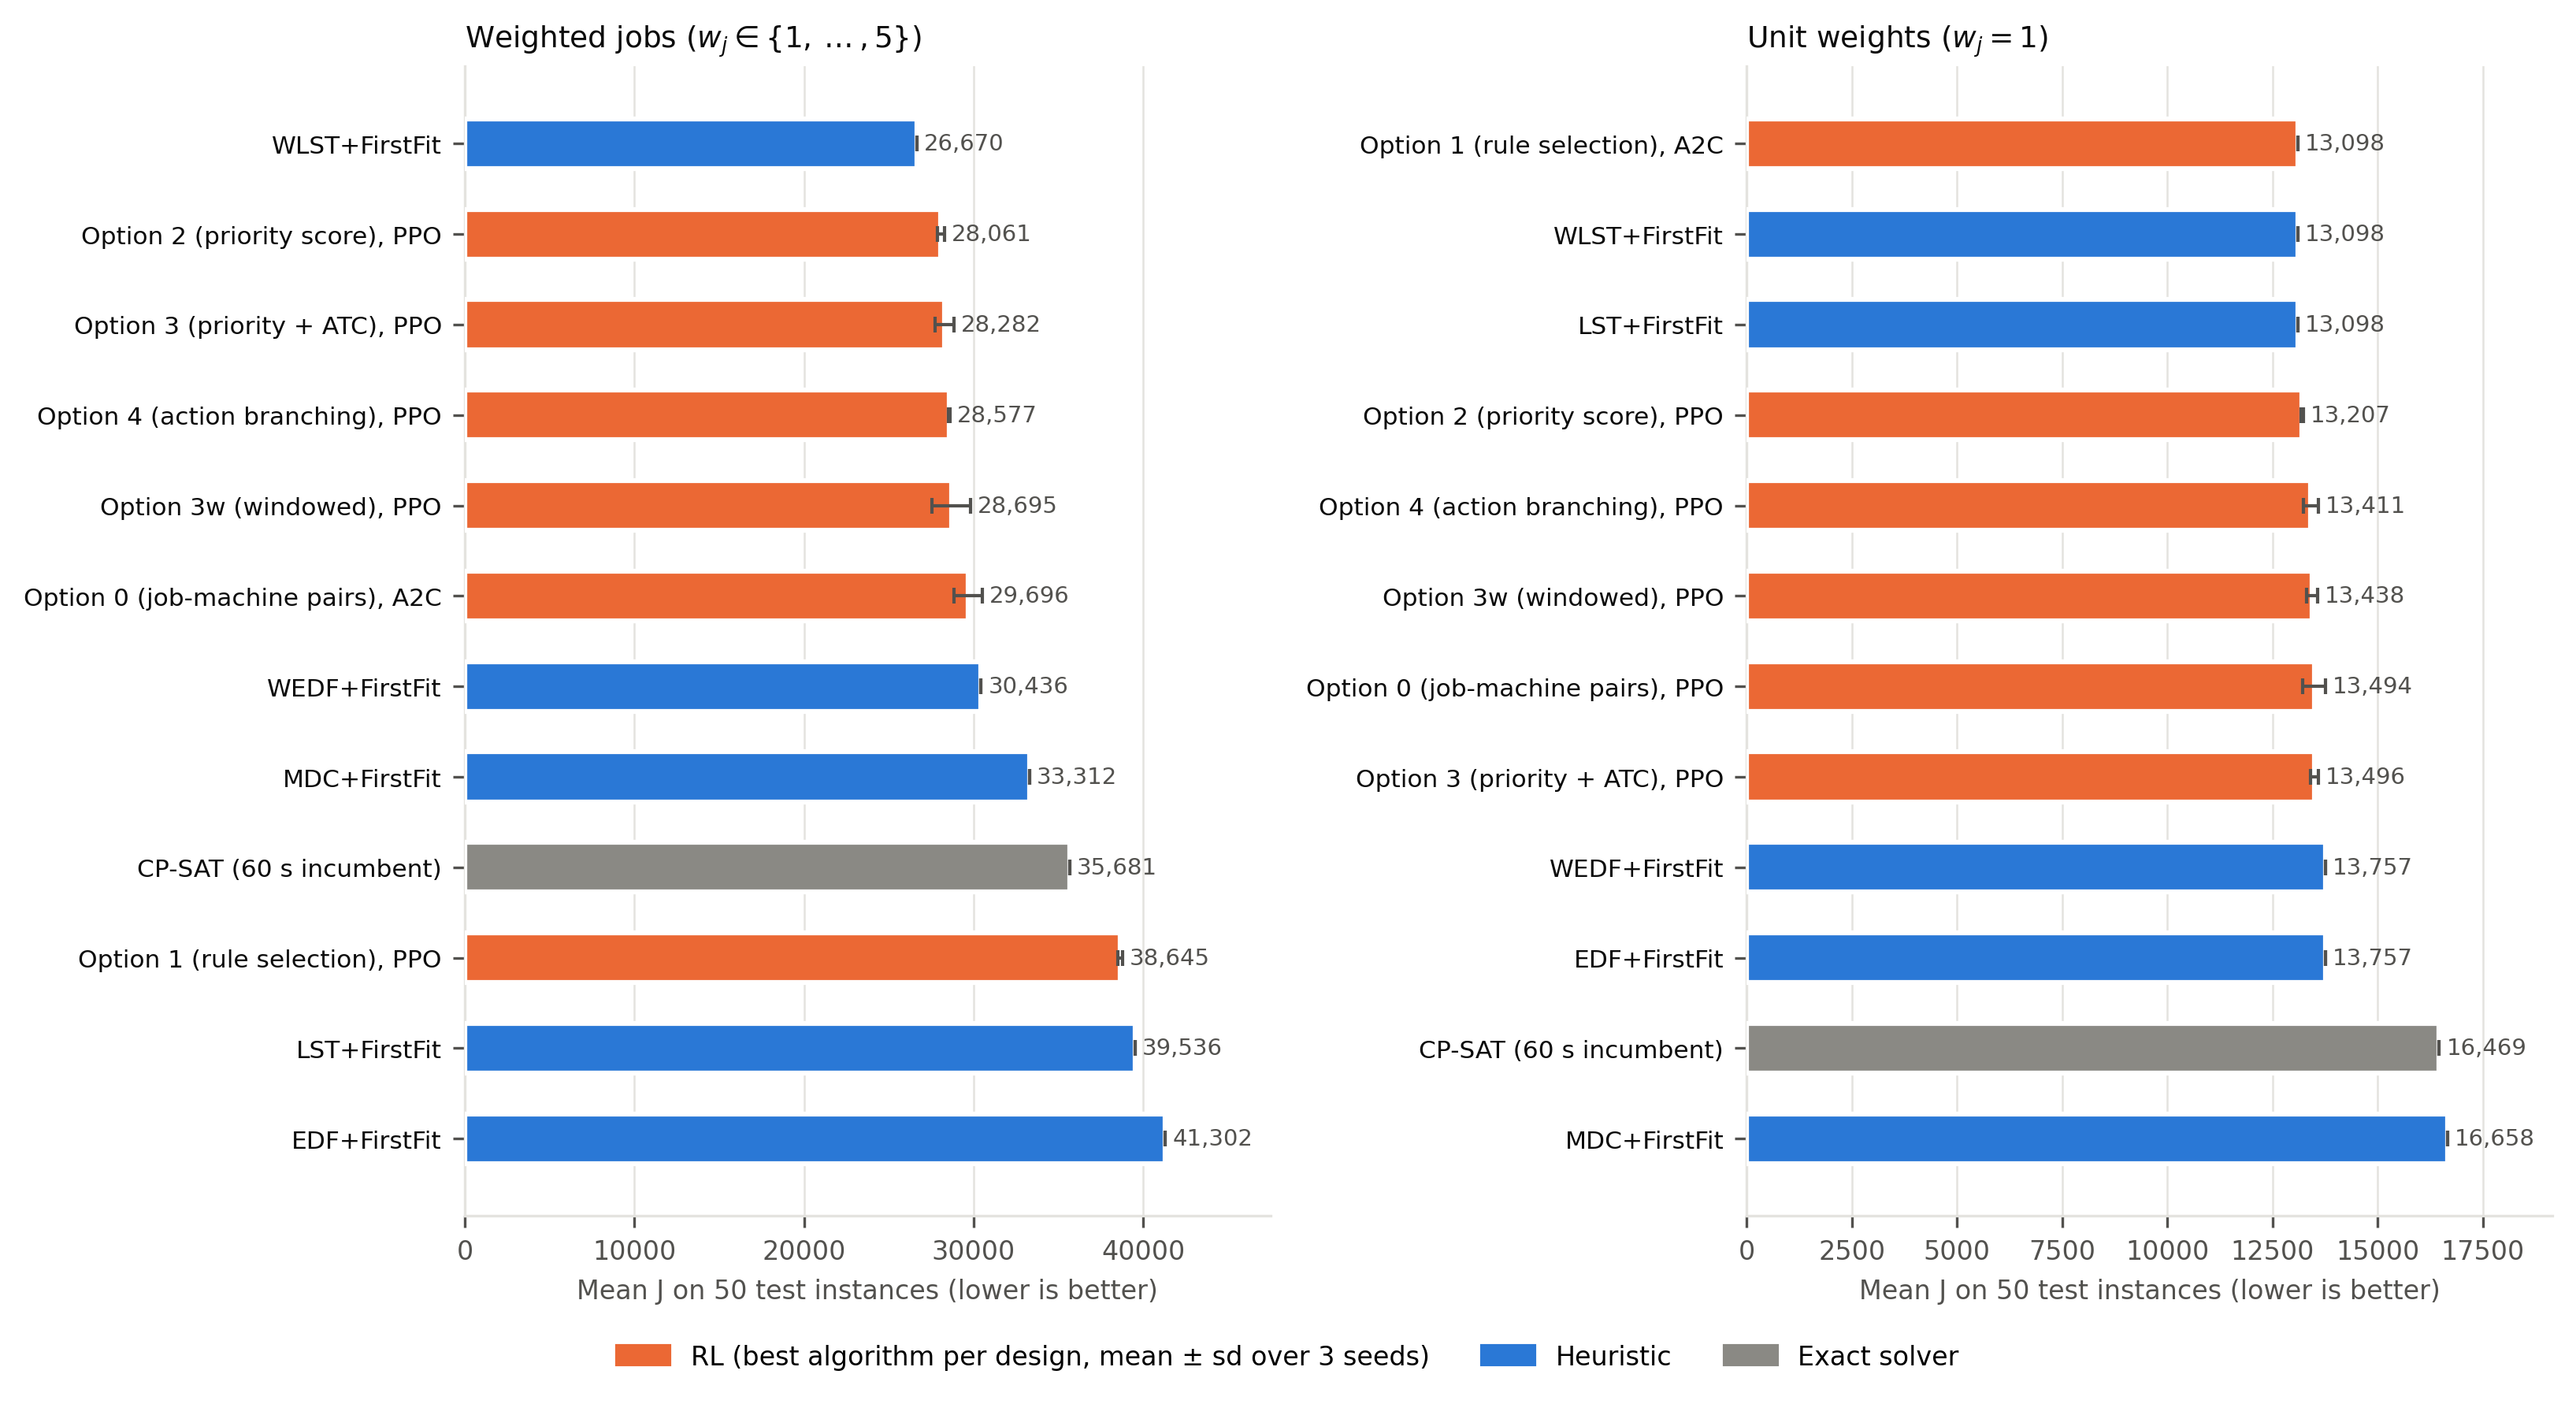
\includegraphics[width=\linewidth]{Images/v2_offline_designs.png}
\caption{\DIFaddFL{Offline results: the best final agent of each design (orange, mean $\pm$ s.d.\ over 3 seeds) against the leading heuristics (blue) and CP-SAT's 60-second schedule (grey). Left: weighted jobs; right: unit weights.}}
\label{fig:offline}
\end{figure}

\subsection{\DIFadd{Combined objectives}}\label{sec:res-mo}
\DIFadd{\mbox{%DIFAUXCMD
\Cref{fig:regime} }\hskip0pt%DIFAUXCMD
answers the research question in one view: for each objective and setting, it compares the best RL agent with the best heuristic. Offline with weighted jobs, RL overtakes }\DIFaddend the best heuristic \DIFdelbegin \DIFdel{, LST, and all of them also scheduled fewer jobs and had more late jobs than LST (\mbox{%DIFAUXCMD
\cref{fig:v1-tard,fig:v1-sched,fig:v1-late}}\hskip0pt%DIFAUXCMD
). The top five methods on reward, tardiness, jobs scheduled and late jobsare shown in \mbox{%DIFAUXCMD
\cref{fig:v1-reward,fig:v1-tard,fig:v1-sched,fig:v1-late}}\hskip0pt%DIFAUXCMD
.

Note that these results are for the constant weight scenario. The uniform weight distribution was only introduced late into v1 and no RL method could beat heuristics.

}\DIFdelend \DIFaddbegin \DIFadd{once the objective rewards more than squared tardiness. Once linear tardiness counts at least as much as the reference ($\times 1$), RL is better by 1.8--10.3\%; with late jobs added at weights $\times 0.5$ to $\times 4$, by 1.4--10.0\%; and with all four terms, by 8.6\%. At moderate weights the winning agents were trained on $J$ alone; at the largest weights, agents trained on the combined objective win. Energy is the exception: RL loses by 3.4--4.8\% at every weight.

}\DIFaddend 

\DIFaddbegin \DIFadd{This advantage depends on job weights and on the setting. With unit weights, RL never beats LST (0.0\% to +10.8\%). Online, RL trails the best heuristic by 5.8--15.7\% on every combined objective.

}

\DIFadd{\mbox{%DIFAUXCMD
\Cref{fig:tradeoff} }\hskip0pt%DIFAUXCMD
shows why RL wins offline. WLST reaches the lowest $J$ by accepting many late jobs (a weighted count of 183). Every heuristic lies on or above the dashed line of the best trade-offs any heuristic achieves, but most RL agents lie below it: for a similar $J$, they finish noticeably more jobs on time. Agents trained on a combined objective (green) move further towards fewer late jobs.

}

\DIFaddend \begin{figure}[htbp]
\centering
\DIFdelbeginFL %DIFDELCMD < \includegraphics[width=0.85\linewidth]{Images/v1_off_c_50_reward_top5.png}
%DIFDELCMD < %%%
\DIFdelendFL \DIFaddbeginFL 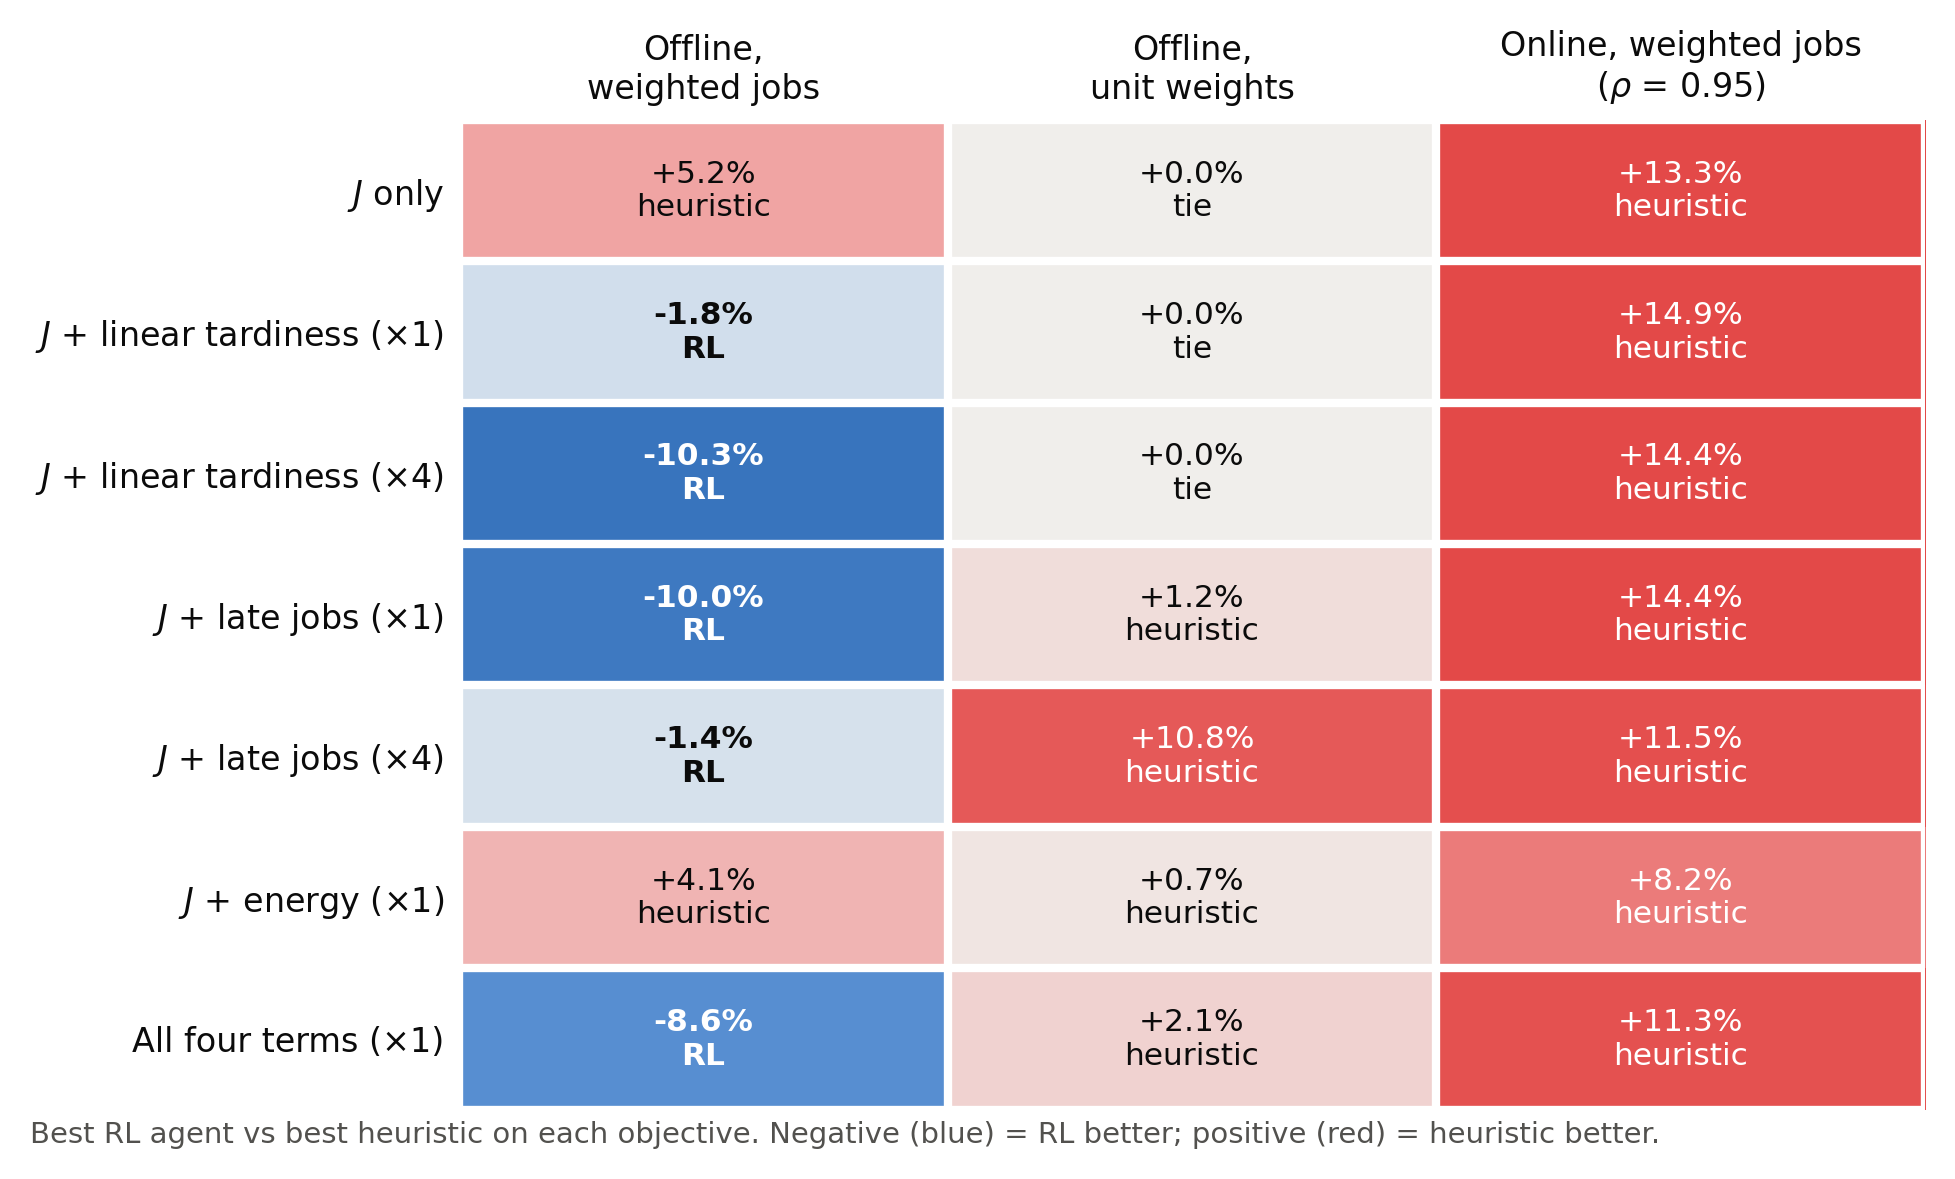
\includegraphics[width=0.85\linewidth]{Images/v2_regime_grid.png}
\DIFaddendFL \caption{\DIFdelbeginFL \DIFdelFL{Top five methods by v1 reward }\DIFdelendFL \DIFaddbeginFL \DIFaddFL{When does RL win? Best RL agent against the best heuristic }\DIFaddendFL on \DIFdelbeginFL \DIFdelFL{50 held-out offline instances }\DIFdelendFL \DIFaddbeginFL \DIFaddFL{each objective }\DIFaddendFL (\DIFdelbeginFL \DIFdelFL{higher }\DIFdelendFL \DIFaddbeginFL \DIFaddFL{rows) and setting (columns); blue means RL }\DIFaddendFL is better\DIFdelbeginFL \DIFdelFL{)}\DIFdelendFL \DIFaddbeginFL \DIFaddFL{, red means the heuristic is better}\DIFaddendFL . \DIFdelbeginFL \DIFdelFL{The two highest-reward methods both have very high tardiness}\DIFdelendFL \DIFaddbeginFL \DIFaddFL{Weights are multiples of the reference values}\DIFaddendFL , \DIFdelbeginFL \DIFdelFL{showing that }\DIFdelendFL \DIFaddbeginFL \DIFaddFL{which make each added term equal to $J$ on }\DIFaddendFL the \DIFdelbeginFL \DIFdelFL{v1 reward did
not measure scheduling quality}\DIFdelendFL \DIFaddbeginFL \DIFaddFL{best heuristic's schedule}\DIFaddendFL . \DIFaddbeginFL \DIFaddFL{Only RL agents with at least two evaluated seeds are included.}\DIFaddendFL }
\DIFdelbeginFL %DIFDELCMD < \label{fig:v1-reward}
%DIFDELCMD < %%%
\DIFdelendFL \DIFaddbeginFL \label{fig:regime}
\DIFaddendFL \end{figure}

\begin{figure}[htbp]
\centering
\DIFdelbeginFL %DIFDELCMD < \includegraphics[width=0.85\linewidth]{Images/v1_off_c_50_tard_top5.png}
%DIFDELCMD < %%%
\DIFdelendFL \DIFaddbeginFL 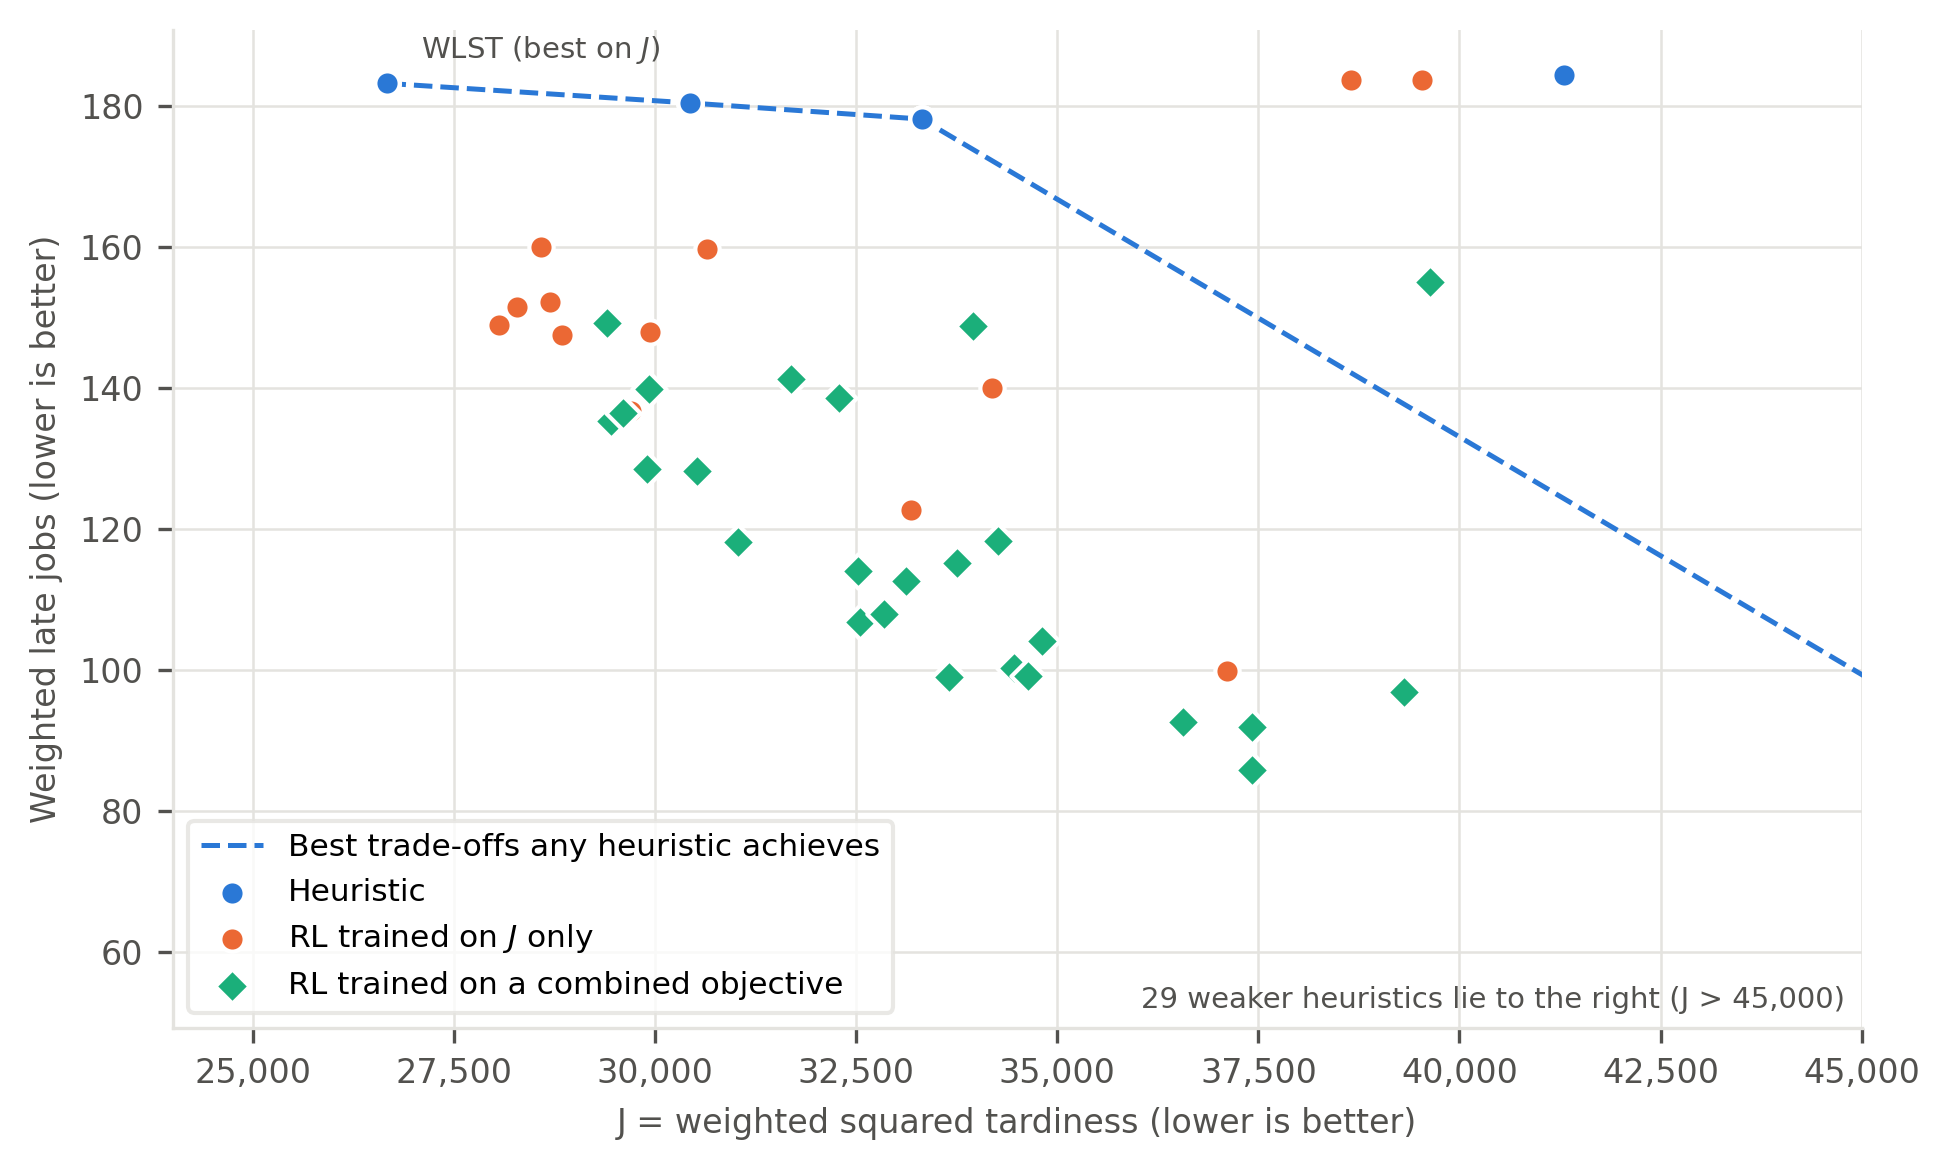
\includegraphics[width=0.85\linewidth]{Images/v2_tradeoff_late.png}
\DIFaddendFL \caption{\DIFdelbeginFL \DIFdelFL{Top five methods by mean total tardiness under v1 }\DIFdelendFL \DIFaddbeginFL \DIFaddFL{Offline, weighted jobs: $J$ against the weighted number of late jobs }\DIFaddendFL (\DIFaddbeginFL \DIFaddFL{both }\DIFaddendFL lower is better) \DIFaddbeginFL \DIFaddFL{for every heuristic and every RL agent with at least two seeds}\DIFaddendFL . The \DIFdelbeginFL \DIFdelFL{only method }\DIFdelendFL \DIFaddbeginFL \DIFaddFL{dashed line joins the best trade-offs among the heuristics; points }\DIFaddendFL below \DIFdelbeginFL \DIFdelFL{LST achieves }\DIFdelendFL it \DIFdelbeginFL \DIFdelFL{by abandoning about 45\% of the jobs}\DIFdelendFL \DIFaddbeginFL \DIFaddFL{achieve combinations no heuristic reaches}\DIFaddendFL .}
\DIFdelbeginFL %DIFDELCMD < \label{fig:v1-tard}
%DIFDELCMD < %%%
\DIFdelendFL \DIFaddbeginFL \label{fig:tradeoff}
\DIFaddendFL \end{figure}

\DIFdelbegin %DIFDELCMD < \begin{figure}[htbp]
%DIFDELCMD < \centering
%DIFDELCMD < \includegraphics[width=0.85\linewidth]{Images/v1_off_c_50_sched_top5.png}
%DIFDELCMD < %%%
%DIFDELCMD < \caption{%
{%DIFAUXCMD
\DIFdelFL{Top five methods by mean number of jobs scheduled, out of 100, under v1 (higher is better). Scheduling nearly every job does not imply they all met
deadlines.}}
%DIFAUXCMD
%DIFDELCMD < \label{fig:v1-sched}
%DIFDELCMD < \end{figure}
%DIFDELCMD < 
%%%
\DIFdelend \DIFaddbegin \subsection{\DIFadd{Online training budget}}\label{sec:res-online}
\DIFadd{More training closes most of the online gap for Option 2 but not for Option 0 (\mbox{%DIFAUXCMD
\cref{tab:budget}}\hskip0pt%DIFAUXCMD
). Option 2's mean $J$ falls from $39{,}947$ at 300k steps to $26{,}515$ at 1M (+21\% over EDF+Consolidate) and $24{,}921$ at 2M (+13\%, 2 seeds), and its best 1M seed is within 4.3\% of the heuristic. Option 0 improves on average but remains 55\% behind at 1M. One Option 2 agent trained for 1M steps on $J$ plus linear tardiness matched EDF+Consolidate ($22{,}000$ vs $21{,}986$), but a second seed of the same setup scored about $30{,}100$, so this was not reproducible. Online A2C did not learn: Option 0 A2C produced the same schedule as FCFS+FirstFit ($J = 44{,}920$) on all three seeds.

}\DIFaddend 

\DIFdelbegin %DIFDELCMD < \begin{figure}[htbp]
%DIFDELCMD < %%%
\DIFdelendFL \DIFaddbeginFL \begin{table}[htbp]
\DIFaddendFL \centering
\DIFdelbeginFL %DIFDELCMD < \includegraphics[width=0.85\linewidth]{Images/v1_off_c_50_late_top5.png}
%DIFDELCMD < %%%
\DIFdelendFL \caption{\DIFdelbeginFL \DIFdelFL{Top five methods by }\DIFdelendFL \DIFaddbeginFL \DIFaddFL{Online ($\rho = 0.95$) }\DIFaddendFL mean \DIFdelbeginFL \DIFdelFL{number of late jobs}\DIFdelendFL \DIFaddbeginFL \DIFaddFL{test $J$ by training budget}\DIFaddendFL , \DIFdelbeginFL \DIFdelFL{out of 100}\DIFdelendFL \DIFaddbeginFL \DIFaddFL{PPO}\DIFaddendFL , \DIFdelbeginFL \DIFdelFL{under v1 }\DIFdelendFL \DIFaddbeginFL \DIFaddFL{mean $\pm$ s.d.\ over seeds }\DIFaddendFL (\DIFdelbeginFL \DIFdelFL{lower is better}\DIFdelendFL \DIFaddbeginFL \DIFaddFL{EDF+Consolidate: 21,986}\DIFaddendFL ).}
\DIFdelbeginFL %DIFDELCMD < \label{fig:v1-late}
%DIFDELCMD < \end{figure}
%DIFDELCMD < 
%%%
\DIFdelend \DIFaddbegin \label{tab:budget}
\begin{tabular}{lrrr}
\toprule
Design & 300k steps & 1M steps & 2M steps \\
\midrule
Option 0 & 49,404 $\pm$ 18,050 & 33,966 $\pm$ 3,699 & -- \\
Option 2 & 39,947 $\pm$ 11,949 & 26,515 $\pm$ 4,564 & 24,921 $\pm$ 2,555 (2 seeds) \\
Option 3 & 44,827 $\pm$ 2,890 & 30,611 $\pm$ 1,909 & -- \\
\bottomrule
\end{tabular}
\end{table}

\DIFaddend 

\DIFdelbegin 
%DIFAUXCMD
\addtocounter{subsubsection}{-1}%DIFAUXCMD
\DIFdel{Similar graphs for the online case are seen in stated github link. In summary, job arrival load $\rho \approx 0.75$ was examined with no RL method outperforming }\DIFdelend \DIFaddbegin \subsection{\DIFadd{Other findings}}\label{sec:res-other}
\paragraph{\DIFadd{Action-space design.}} \DIFadd{Learning a job priority (Options 2 and 3) worked best in every setting. Picking job-machine pairs directly (Option 0) was 6\% worse offline and still 55\% behind online after 1M steps, and choosing job and machine with two heads (Option 4), competitive offline, failed online ($J = 139{,}721$). Rule selection (Option 1) mostly collapsed onto a single rule: with unit weights it reproduced LST exactly on all three seeds, and with weighted jobs its schedules had the same number of late jobs as LST (61.0) and a similar $J$ (within 2.3\% of LST).

}

\paragraph{\DIFadd{Training stability.}} \DIFadd{In 8 independent offline runs of the same Option 2 configuration (default hyperparameters, 300k steps), one diverged ($J = 69{,}367$ against $28{,}352$--$30{,}925$ for the other seven). Online seeds differ much more: Option 2 at 300k steps ranged from $30{,}076$ to $53{,}231$.

}

\paragraph{\DIFadd{Energy.}} \DIFadd{RL lost to }\DIFaddend the best heuristic \DIFdelbegin \DIFdel{in either constant weightsor uniform weight distribution. }\DIFdelend \DIFaddbegin \DIFadd{(WLST+Consolidate) on every $J$ + energy objective, by 3.4--4.8\%. Training with the energy term made no run diverge in 8 seeds, but it did not make training meaningfully more stable either: those runs were 5--25\% worse on $J$, the expected cost of trading $J$ for energy.

}\DIFaddend 

\DIFdelbegin 

%DIFAUXCMD
\addtocounter{subsection}{-1}%DIFAUXCMD
\DIFdelend \DIFaddbegin \paragraph{\DIFadd{No single heuristic wins everywhere.}} \DIFadd{The best rule changed with deadline tightness and load: EDF with loose offline deadlines (TF $= 0.2$, where it reaches $J = 0$), WLST with medium and tight deadlines, LST with unit weights, WLST+Consolidate online at $\rho = 0.50$ and $0.75$, EDF+Consolidate at $\rho = 0.95$, and MDC+Consolidate under overload ($\rho = 1.10$). Online, Consolidate placement was best at every load.

}\DIFaddend 

\DIFaddbegin \paragraph{\DIFadd{Hyperparameter tuning.}} \DIFadd{The library defaults were the best configuration in 8 of the 24 studies, including both studies for Options 0 and 2 PPO online that were stopped early.

}

%DIF >  =====================================================================
\DIFaddend \section{Discussion}\DIFaddbegin \label{sec:discussion}
\paragraph{\DIFadd{When does RL beat the heuristics?}} \DIFadd{Our results suggest three conditions. First, }\emph{\DIFadd{the objective must not be one that a simple rule already solves well}}\DIFadd{. With unit weights and squared tardiness, LST matched every proven optimum on small instances, and RL could at best reproduce it. When the objective mixes several goals (\mbox{%DIFAUXCMD
\cref{sec:res-mo}}\hskip0pt%DIFAUXCMD
), no single rule is designed for the combination, and RL won by up to 10\%. Second, }\emph{\DIFadd{jobs must differ in importance}}\DIFadd{. The offline multi-objective advantage disappeared with unit weights. Weights give a learned priority more to work with, since the right order now depends jointly on deadline, length and weight. This condition was tested offline only, because every online setting used weighted jobs. Third, }\emph{\DIFadd{the agent must be trained enough for the setting}}\DIFadd{. Offline, 1M steps was enough to come within 5\% of the best heuristic. Online, 300k steps left RL 70\% behind, and 1--2M steps closed most of the gap for the best design.

}\DIFaddend 

\DIFaddbegin \paragraph{\DIFadd{RL and heuristic design.}} \DIFadd{The best offline heuristic, WLST, did not exist at the start of the project: it was constructed after RL agents had beaten every published rule by 29\%. One reading is that RL lost to WLST. A fairer reading is that RL found, automatically and within 5\%, a level of performance that took a purpose-built rule to match. This suggests that RL could also serve as a tool for heuristic design, by revealing that better rules exist for a new objective. It also shows how much results depend on the choice of baselines. Studies that compare RL only with standard rules would have reported a clear RL win here.

}

\paragraph{\DIFadd{Why the multi-objective gains need care.}} \DIFadd{At moderate weights, the agents that won the composite objectives were trained on $J$ alone. Their schedules happened to have fewer late jobs and lower linear tardiness than WLST's (for example, Option 0 A2C: 52.7 late jobs against 61.7; \mbox{%DIFAUXCMD
\cref{fig:tradeoff}}\hskip0pt%DIFAUXCMD
). WLST is tuned for squared tardiness and gives up the other metrics to get it. This part of the advantage is therefore a side effect of how RL schedules, not a trade-off it learned, and it is exactly the kind of pattern in non-optimised metrics that must not be over-interpreted. At larger weights, agents trained on the composite objective took over, which does indicate learning. Re-running these agents with the tuned settings and full 1M-step budget is in progress.

}

\paragraph{\DIFadd{Why online is harder.}} \DIFadd{Online returns depend heavily on the random arrival sequence, which the agent cannot predict, so the training signal is much noisier than offline \mbox{%DIFAUXCMD
\cite{mao2019variance}}\hskip0pt%DIFAUXCMD
. Online episodes are also roughly ten times longer, and the observation has to cover over a thousand job slots. Both effects mean more samples are needed, consistent with the budget results. Option 0's much larger action space compounds the problem \mbox{%DIFAUXCMD
\cite{dulacarnold2015largeactionspaces}}\hskip0pt%DIFAUXCMD
.

}

\paragraph{\DIFadd{Action spaces and energy.}} \DIFadd{Priority learning worked best, in line with DeepRM and Decima, which also let the network choose the job and leave placement to the system \mbox{%DIFAUXCMD
\cite{mao2016deeprm, mao2019decima}}\hskip0pt%DIFAUXCMD
. Rule selection collapsed onto one rule, so it can at best match the best rule in its menu. Options 2 and 3 always place with First-Fit and so cannot consolidate jobs onto fewer machines, a likely (still untested) reason they lose on energy.

}

\paragraph{\DIFadd{Practical considerations.}} \DIFadd{RL training is unstable (one diverged run in eight) and expensive, and tuning helped little: the defaults were best in 8 of 24 studies, consistent with the known sensitivity of RL to hyperparameters and the small tuning budgets typically used \mbox{%DIFAUXCMD
\cite{eimer2023hyperparams}}\hskip0pt%DIFAUXCMD
. A heuristic needs no training and behaves the same every time. RL is therefore worth its cost mainly where the objective is complex and weighted, and where enough compute is available.

}

\paragraph{\DIFadd{Limitations.}} \DIFadd{All instances are synthetic and of one size (100 jobs, 10 machines), and results use 3 seeds. Picking the best of many RL variants on the test set slightly favours RL, although the best heuristic is picked the same way. CP-SAT did not reach optimality at 100 jobs, so the distance of RL and WLST from the optimum is unknown. The online 2M-step results rest on two seeds, and three online studies were stopped early.

}

%DIF >  =====================================================================
\DIFaddend \section{Conclusion}\DIFaddbegin \label{sec:conclusion}
\DIFadd{This project formulated cloud resource allocation as a multi-resource scheduling problem and an MDP, built an offline and online simulation environment, and compared six RL action-space designs, trained with PPO and A2C under one uniform protocol, against 49 heuristics and an exact solver. On the main objective, weighted squared tardiness, RL came within 5\% of the best heuristic offline and beat every published rule by 29\%, but did not beat the best rule, which was purpose-built for that objective. RL did beat the best heuristic, by 2--10\%, once linear tardiness or late jobs were added to the objective, provided jobs had different weights. Online, RL needed several times more training to approach the heuristics, and it never won when energy was part of the objective. Learning a job priority was the most effective design. Getting RL to train reliably required careful diagnosis: reward scaling and event-driven idling were essential. In short, RL is most competitive when the objective combines goals that no single rule targets, jobs differ in importance, and training is sufficient. Where a simple rule is already near-optimal, the heuristic remains the better choice.

}\DIFaddend 

\section{Future Work}
\begin{itemize}
    \item \DIFdelbegin \DIFdel{More research and consideration into the online case. The online case remains incredibly complex and this projectonly touches on it briefly. }\DIFdelend \DIFaddbegin \DIFadd{Extend the online study with longer training and more seeds, since the online gap was mainly a training-budget problem.
    }\DIFaddend \item \DIFdelbegin \DIFdel{Look more into hybrid architectures \mbox{%DIFAUXCMD
\cite{ml_ra_litrev2025}
    }\hskip0pt%DIFAUXCMD
}\DIFdelend \DIFaddbegin \DIFadd{Test generalisation to other deadline tightness and loads (in progress), larger clusters, and real traces such as Google's \mbox{%DIFAUXCMD
\cite{reiss2012googletrace} }\hskip0pt%DIFAUXCMD
or Azure's \mbox{%DIFAUXCMD
\cite{cortez2017resourcecentral}}\hskip0pt%DIFAUXCMD
.
    }\DIFaddend \item \DIFdelbegin \DIFdel{Adopt simulation-based training and interactive learning environments \mbox{%DIFAUXCMD
\cite{ml_ra_litrev2025}
    }\hskip0pt%DIFAUXCMD
}\DIFdelend \DIFaddbegin \DIFadd{Let RL choose placement as well as job order, e.g.\ with a consolidating placement rule, to address the energy gap.
    }\DIFaddend \item \DIFdelbegin \DIFdel{Considering more and different metrics and objectives
    }\DIFdelend \DIFaddbegin \DIFadd{Train one agent conditioned on the objective weights \mbox{%DIFAUXCMD
\cite{abels2019dynamicweights, hayes2022morlguide}}\hskip0pt%DIFAUXCMD
, and try graph neural network encoders \mbox{%DIFAUXCMD
\cite{gnn2024jsspsurvey}}\hskip0pt%DIFAUXCMD
.
    }\DIFaddend \item \DIFdelbegin \DIFdel{Examine the large action-space failure of policy-based methods, and evaluate how different methods compare and potentially aid in this project's future findings.

This includes replacing the current pointer network encoding with graph neural networks for job /machine encoding \mbox{%DIFAUXCMD
\cite{gnn2024jsspsurvey}}\hskip0pt%DIFAUXCMD
, and a variety of action-space reductions and branching \mbox{%DIFAUXCMD
\cite{tavakoli2018actionbranching}
    }\hskip0pt%DIFAUXCMD
}%DIFDELCMD < \item %%%

\DIFdel{Evaluate large discrete action space methods such as the Wolpertinger architecture \mbox{%DIFAUXCMD
\cite{dulacarnold2015largeactionspaces}
    }\hskip0pt%DIFAUXCMD
}%DIFDELCMD < \item %%%

\DIFdel{Investigate more improvements to many models like RCPO, ATC dispatching, rule-selection and other algorithms implemented
    }%DIFDELCMD < \item %%%

\DIFdel{Evaluate the trained policies against real-world data from e.
    g Googlecluster trace or Microsoft Azuretrace
    }%DIFDELCMD < \item %%%

\DIFdel{Conduct a formulation and environmental review of problem structure for different goals.
Many small changes can be made that may increase performance
}\DIFdelend \DIFaddbegin \DIFadd{Use RL for heuristic discovery: extract interpretable rules from learned priorities.
}\DIFaddend \end{itemize}

\DIFdelbegin %DIFDELCMD < \newpage
%DIFDELCMD < %%%

%DIFAUXCMD
\addtocounter{section}{-1}%DIFAUXCMD
\DIFdel{Your task is to:
}%DIFDELCMD < \newline
%DIFDELCMD < %%%
\DIFdel{Write a report of approximately 3000 – 5000 words (excluding gures, captions, references, tables, and appendices)that details your activities through this unit. The content and layout of your report will depend on the type of project/s you undertook as part of this unit. A combination of visual and textual information should be included in the report. The format of reports may vary across discipline areas.

While each report will be unique in terms of focus and outcomes, the following sections should be included:
}\DIFdelend %DIF >  =====================================================================
\DIFaddbegin \section*{\DIFadd{Data Management Plan}}
\DIFadd{All code, raw results (per-instance metrics for every method and seed), processed tables and figures, Optuna study logs and the chronological experiment log are in the public GitHub repository}\footnote{\url{https://github.com/Ethan-Ty-Riekert/Neural-Knapsack-Research-Project}}\DIFadd{. Results are under }\texttt{\DIFadd{Results/}} \DIFadd{(raw runs, tuning studies, and the processed }\texttt{\DIFadd{ALL\_RESULTS}} \DIFadd{archive), and every number in this report can be regenerated from them with the scripts provided. All instances are synthetic and generated from fixed random seeds, so no personal or sensitive data is involved. Trained model files are regenerated by the training scripts and are not version-controlled. The version cited in this report is a tagged release on the }\texttt{\DIFadd{main}} \DIFadd{branch.

}\DIFaddend 

\DIFaddbegin \section*{\DIFadd{Generative AI Use Statement}}
\DIFadd{Claude Code (Anthropic) was used as a coding and research assistant. The original environment and the translation of the mathematical formulation into code were done by hand. Claude Code was used to implement models, training and evaluation, and to run experiments, under the following rules:
}\DIFaddend \begin{itemize}
    \DIFdelbegin %DIFDELCMD < \item %%%

\DIFdel{A succinct title that reects the focus of the project
    }\DIFdelend \item \DIFdelbegin \DIFdel{Your name, your supervisor’s name(s)}\DIFdelend \DIFaddbegin \textbf{\DIFadd{Context.}} \DIFadd{Claude was given the latest version of the report, formulations and experiment logs.
    }\DIFaddend \item \DIFdelbegin \DIFdel{Concise introduction to your project which orientates the reader (Abstract)}\DIFdelend \DIFaddbegin \textbf{\DIFadd{Rules.}} \DIFadd{Every design decision had to be cited and justified, or derived, and implementation and discussion had to remain mathematically grounded.
    }\DIFaddend \item \DIFdelbegin \DIFdel{Project aims/goals/objectives
    }\DIFdelend \DIFaddbegin \textbf{\DIFadd{Benchmarking and results.}} \DIFadd{Experiments were run by Claude from a queue, and every result was reviewed personally.
    }\DIFaddend \item \DIFdelbegin \DIFdel{Specific project outputs/deliverables
    }\DIFdelend \DIFaddbegin \textbf{\DIFadd{Diagnostics and research.}} \DIFadd{Unexpected results and failures were investigated and checked against the literature.
    }\DIFaddend \item \DIFdelbegin \DIFdel{Background : reference to literature justifying the value and importance of the project
    }%DIFDELCMD < \item %%%

\DIFdel{Methodology
    }%DIFDELCMD < \item %%%

\DIFdel{Results: Present results in a format relevant to your discipline. Use graphical and tabular format where appropriate.
    }%DIFDELCMD < \item %%%

\DIFdel{Discussion – what you achieved/discovered, the relevance of what you achieved
    }%DIFDELCMD < \item %%%

\DIFdel{Conclusion
    }%DIFDELCMD < \item %%%

\DIFdel{Future projects that may build on this project or new ideas for future projects emerging from your work this year
}\DIFdelend \DIFaddbegin \textbf{\DIFadd{Recording.}} \DIFadd{Every decision and result was recorded in an experiment log.
}\DIFaddend \end{itemize}
\DIFaddbegin \DIFadd{All modelling decisions and formulations were reviewed and approved personally. Using Claude allowed far more experiments, analyses and model iterations than would otherwise have been possible, and made it easier to discuss modelling decisions against other papers. Separate Claude agents were also used weekly to check the code's efficiency, mathematical rigour and factual accuracy. Claude was also used to help edit the text of this report; all content was reviewed and approved by the author.

}\DIFaddend 

\DIFdelbegin \DIFdel{Not included in the word count, but must be included:

}%DIFDELCMD < 

%DIFDELCMD < %%%
\DIFdel{Data Management Plan -- access to raw data, processed data, code repository
GenAI use statement - declare use of any GenAI software and how it was used .
References
}\DIFdelend \newpage
%DIF < \nocite{*}
\bibliographystyle{IEEEtran}
%DIF <  \bibliographystyle{IEEEtranSN}
\bibliography{references}

\newpage
\DIFdelbegin 

%DIFAUXCMD
\addtocounter{section}{-1}%DIFAUXCMD
%DIFDELCMD < 

%DIFDELCMD < 
%DIFDELCMD < 
%DIFDELCMD < %%%

\addtocounter{subsection}{-1}%DIFAUXCMD
\DIFdelend \DIFaddbegin \appendix
\section{\DIFadd{Nomenclature}}\DIFaddend \label{sec:AppendixA}
\begin{table}[htbp]
\centering
\caption{Nomenclature}
\label{tab:nomenclature}
\DIFdelbeginFL %DIFDELCMD < \begin{tabular}{ll}
%DIFDELCMD < \hline
%DIFDELCMD < \multicolumn{2}{l}{\textbf{Sets}}\\
%DIFDELCMD < \hline
%DIFDELCMD < $J$ & Set of jobs, indexed by $j$ \\
%DIFDELCMD < $P$ & Set of processing jobs \\
%DIFDELCMD < $J_t$ & Jobs currently waiting (not yet started) at time $t$ \\
%DIFDELCMD < $M$ & Set of candidate machines, indexed by $m$ \\
%DIFDELCMD < $R$ & Set of resource types, indexed by $r$ \\
%DIFDELCMD < $\mathcal{T}$ & Set of discrete time periods, indexed by $t$ \\
%DIFDELCMD < \hline
%DIFDELCMD < \multicolumn{2}{l}{\textbf{Parameters}}\\
%DIFDELCMD < \hline
%DIFDELCMD < $p_j$ & Processing duration of job $j$ \\
%DIFDELCMD < $a_{jr}$ & Requirement of job $j$ for resource type $r$ \\
%DIFDELCMD < $C_r$ & Capacity of each machine for resource type $r$ \\
%DIFDELCMD < $H$ & Length of the planning horizon \\
%DIFDELCMD < $d_j$ & Due date or deadline of job $j$ \\
%DIFDELCMD < $w_j$ & Priority weight or penalty weight of job $j$ \\
%DIFDELCMD < $\tau_j$ & Arrival time of job $j$ (for offline is $0$) \\
%DIFDELCMD < $\nu$, $\rho$ & Arrival rate and load factor for online jobs \\
%DIFDELCMD < $\lambda_1,\lambda_2,\lambda_3$ & Weights in the v1 objective \\
%DIFDELCMD < $\lambda_S,\lambda_T,\lambda_U,\lambda_E$ & Weights in the v2 objective \\
%DIFDELCMD < \hline
%DIFDELCMD < \multicolumn{2}{l}{\textbf{Decision variables}}\\
%DIFDELCMD < \hline
%DIFDELCMD < $x_{jmt}$ & 1 if job $j$ starts on machine $m$ at time $t$; 0 otherwise \\
%DIFDELCMD < $y_m$ & 1 if machine $m$ is used; 0 otherwise \\
%DIFDELCMD < $s_j$ & Start time of job $j$ \\
%DIFDELCMD < $T_j$ & Tardiness of job $j$ \\
%DIFDELCMD < $U_{mrt}$ & Total usage of resource $r$ on machine $m$ at time $t$ \\
%DIFDELCMD < $\theta$ & Maximum utilisation ratio over all machines, resources, and time periods \\
%DIFDELCMD < \hline
%DIFDELCMD < \end{tabular}
%DIFDELCMD < %%%
\DIFdelendFL \DIFaddbeginFL \begin{tabular}{ll}
\toprule
\multicolumn{2}{l}{\textbf{Sets}}\\
\midrule
$J$ & Set of jobs, indexed by $j$ \\
$J_t$ & Jobs waiting (arrived, not yet started) at time $t$ \\
$P_t$ & Jobs processing (started, not finished) at time $t$ \\
$M$ & Set of machines, indexed by $m$ \\
$R$ & Set of resource types, indexed by $r$ \\
$\mathcal{T}$ & Set of discrete time periods, indexed by $t$ \\
\midrule
\multicolumn{2}{l}{\textbf{Parameters}}\\
\midrule
$p_j$ & Processing duration of job $j$ \\
$a_{jr}$ & Requirement of job $j$ for resource $r$ \\
$C_r$ & Capacity of each machine for resource $r$ \\
$H$ & Length of the planning horizon \\
$d_j$ & Due date of job $j$ \\
$w_j$ & Priority weight of job $j$ \\
$\tau_j$ & Arrival time of job $j$ ($0$ offline) \\
$\nu$, $\rho$ & Arrival rate and load factor (online) \\
TF, RDD & Tardiness factor and due-date range (offline deadlines) \\
$\lambda_1, \lambda_2, \lambda_3$ & Weights in the initial objective \cref{eq:objective-v1} \\
$\lambda_T, \lambda_U, \lambda_E$ & Weights in the final objective \cref{eq:objective-v2} \\
\midrule
\multicolumn{2}{l}{\textbf{Decision variables}}\\
\midrule
$x_{jmt}$ & 1 if job $j$ starts on machine $m$ at time $t$; 0 otherwise \\
$y_m$ & 1 if machine $m$ is used; 0 otherwise \\
$s_j$ & Start time of job $j$ \\
$T_j$ & Tardiness of job $j$, $\max(0, s_j + p_j - d_j)$ \\
$U_j$ & 1 if job $j$ finishes after $d_j$; 0 otherwise \\
$E$ & Energy: total active machine-time \\
$U_{mrt}$ & Total usage of resource $r$ on machine $m$ at time $t$ \\
$\theta$ & Peak utilisation ratio, $\max_{m,r,t} U_{mrt}/C_r$ \\
\bottomrule
\end{tabular}
\DIFaddendFL \end{table}

\DIFdelbegin 
\addtocounter{subsection}{-1}%DIFAUXCMD
\DIFdelend \DIFaddbegin \section{\DIFadd{Constraints}}\DIFaddend \label{sec:AppendixB}
\DIFaddbegin \DIFadd{Let $\mathcal{T} = \{0, 1, \dots, \bar{H}\}$, where $\bar{H}$ is any upper bound on the time to finish all jobs (e.g.\ $H + \sum_j p_j$, under the extended horizon). For each job, let $\mathcal{T}_j = \{t \in \mathcal{T} : \tau_j \le t \le \bar{H} - p_j\}$ be its feasible start times.

}

\paragraph{\DIFadd{Assignment.}} \DIFadd{Each job starts exactly once, on exactly one machine, and never before it arrives:
}\begin{equation}\DIFadd{\label{con:assign}
    \sum_{m \in M} \sum_{t \in \mathcal{T}_j} x_{jmt} = 1, \qquad \forall j \in J.
}\end{equation}
\paragraph{\DIFadd{Offline start rate.}} \DIFadd{Offline, at most one job starts per time step:
}\begin{equation}\DIFadd{\label{con:one-start}
    \sum_{j \in J} \sum_{m \in M} x_{jmt} \le 1, \qquad \forall t \in \mathcal{T}.
}\end{equation}
\paragraph{\DIFadd{Machine activation.}} \DIFadd{A job can only be placed on an active machine:
}\begin{equation}\DIFadd{\label{con:machine-use}
    x_{jmt} \le y_m, \qquad \forall j \in J,\ m \in M,\ t \in \mathcal{T}_j.
}\end{equation}
\paragraph{\DIFadd{Start time.}}
\begin{equation}\DIFadd{\label{con:start-time}
    s_j = \sum_{m \in M} \sum_{t \in \mathcal{T}_j} t\, x_{jmt}, \qquad \forall j \in J.
}\end{equation}
\paragraph{\DIFadd{Resource usage and capacity.}} \DIFadd{A job started at $t'$ occupies its resources during $[t', t'+p_j)$, so the usage at time $t$ counts every job started within the previous $p_j$ steps. Usage may never exceed capacity:
}\begin{equation}\DIFadd{\label{con:resource-usage}
    U_{mrt} = \sum_{j \in J} \; \sum_{\substack{t' \in \mathcal{T}_j \\ t - p_j < t' \le t}} a_{jr}\, x_{jmt'} \;\le\; C_r, \qquad \forall m \in M,\ r \in R,\ t \in \mathcal{T}.
}\end{equation}
\paragraph{\DIFadd{Tardiness, late jobs and peak utilisation.}}
\begin{equation}\DIFadd{\label{con:tardiness}
    T_j \ge s_j + p_j - d_j, \quad T_j \ge 0, \quad T_j \le \bar{H}\, U_j, \qquad \forall j \in J,
}\end{equation}
\begin{equation}\DIFadd{\label{con:theta}
    \theta \ge \frac{U_{mrt}}{C_r}, \qquad \forall m \in M,\ r \in R,\ t \in \mathcal{T}.
}\end{equation}
\DIFadd{Because the objectives are minimised and increase with $T_j$, $U_j$ and $\theta$, these inequalities hold with equality at the optimum. Finally, $x_{jmt}, y_m, U_j \in \{0, 1\}$.

}

\section{\DIFadd{Hyperparameter Search Space}}\label{sec:AppendixC}
\begin{table}[htbp]
\centering
\caption{\DIFaddFL{Hyperparameters searched by Optuna (ranges after \mbox{%DIFAUXCMD
\cite{andrychowicz2021onpolicy}}\hskip0pt%DIFAUXCMD
). ``log'' means sampled log-uniformly; lists are categorical choices. Trial 0 of every study used the library defaults instead.}}
\label{tab:hp}
\begin{tabular}{lll}
\toprule
Hyperparameter & PPO & A2C \\
\midrule
Learning rate & $3\times10^{-5}$ -- $10^{-3}$ (log) & $10^{-4}$ -- $3\times10^{-3}$ (log) \\
Rollout length (all 4 environments) & 2048, 4096, 8192, 16384 & 20, 80, 320 \\
Minibatch size & 64, 256, 1024 & -- \\
Epochs per update & 3, 5, 10 & -- \\
Discount factor $\gamma$ & 0.99, 0.995, 0.999 & 0.99, 0.995, 0.999 \\
GAE $\lambda$ & 0.9, 0.95, 0.98 & 0.9, 0.95, 1.0 \\
Clip range & 0.1, 0.2, 0.3 & -- \\
Entropy coefficient & $10^{-4}$ -- $3\times10^{-2}$ (log) & $10^{-4}$ -- $3\times10^{-2}$ (log) \\
\bottomrule
\end{tabular}
\end{table}

\section{\DIFadd{Experimental Details}}\label{sec:AppendixD}
\paragraph{\DIFadd{Offline deadlines.}} \DIFadd{Following Potts and Van Wassenhove \mbox{%DIFAUXCMD
\cite{potts1985wtardiness}}\hskip0pt%DIFAUXCMD
, each $d_j$ is drawn uniformly from $[\,\bar{C}(1 - \mathrm{TF} - \mathrm{RDD}/2),\ \bar{C}(1 - \mathrm{TF} + \mathrm{RDD}/2)\,]$ and is at least $p_j$. Here $\bar{C}$ is a lower bound on the time to finish all jobs (the larger of the number of jobs, since one job starts per step, and the total work divided by the cluster's capacity), TF is the tardiness factor and RDD $= 0.6$ the range of due dates, which sets how spread out deadlines are.

}

\paragraph{\DIFadd{Online deadlines and job sizes.}} \DIFadd{A job's deadline is its arrival time plus a slack drawn uniformly from $\{10, \dots, 60\}$ time steps ($\{5, \dots, 25\}$ in a tight-deadline variant). Durations and demands are log-normal, not Gaussian: the logarithm of the size is normally distributed (with $\sigma = 1$), giving many small jobs and a few large ones. The location parameter is set so that the mean equals that of the offline uniform distribution, and sizes are capped at four times the offline maximum (durations of at most 40 steps).

}

\paragraph{\DIFadd{Tuning protocol.}} \DIFadd{Each of the 24 studies ran 12 trials of 300,000 steps with 4 parallel environments; trial 0 used the Stable-Baselines3 defaults, which lie outside the log-scaled search space (the default entropy coefficient is 0). Every 75,000 steps, a trial reported its mean $J$ on 5 validation instances. Optuna's median pruner stopped the trial if this was worse than the median of the values earlier trials had reported at the same step; pruning only starts after 5 trials have finished. A completed trial's score is its mean $J$ on all 20 validation instances, and the best score gives the study's single chosen configuration. The offline configuration was reused for the unit-weight setting. Three online PPO studies (Options 0, 2 and 4) trained at about 20 steps per second, roughly 4--5 hours per trial, and were stopped after 3--7 trials to meet the project deadline; the best completed trial was used as usual. The defaults were the best configuration in 8 of the 24 studies.

}

\paragraph{\DIFadd{Faults fixed in the final training version.}} \DIFadd{Each fault was measured directly in training logs.
}\begin{enumerate}[nosep]
    \item \emph{\DIFadd{The critic did not learn.}} \DIFadd{Squared-tardiness returns are in the hundreds to thousands, and the value and policy losses share one clipped gradient, so the value error swamped each update. The critic explained none of the variance in returns, and A2C policies stayed close to uniformly random. Rewards are now divided by a running estimate of the standard deviation of the return \mbox{%DIFAUXCMD
\cite{engstrom2020implementation, andrychowicz2021onpolicy}}\hskip0pt%DIFAUXCMD
; afterwards the critic explained 30--99.9\% of the variance.
    }\item \emph{\DIFadd{Deterministic evaluation idled.}} \DIFadd{Idle is a single action, while the probability of starting a job is split across many (job, machine) actions. For an undecided policy, idle could be the single most likely action in every state, so a ``most likely action'' rule idled indefinitely even though the trained (sampling) policy placed jobs 98\% of the time. The two-stage rule of \mbox{%DIFAUXCMD
\cref{sec:evaluation} }\hskip0pt%DIFAUXCMD
fixes this, and is identical to the most-likely-action rule for confident policies.
    }\item \emph{\DIFadd{Idling could repeat forever.}} \DIFadd{An idle used to advance time by one step and return the agent to an unchanged decision. Event-driven idling advances to the next arrival or completion instead. Waiting between events never helps, since a job that fits at an intermediate step also fits now and finishes earlier, so no schedule is lost.
}\end{enumerate}
\DIFadd{Together, these changes reduced offline Option 0 A2C's validation $J$ from 234,116 to 43,164.

}\DIFaddend 

\end{document}
